\documentclass[12pt,a4paper,openright,oneside]{book}

%------------------------------------------------------------------------------%
%                                                                              %
%   LaTeX Template for Bachlor Thesis of Northwestern Polytechnical University %
%   Using XeLeTeX + MakeIndex + BibTeX, or Using CTeX v2.9.2.164               %
%   Version: 1.3.0                                                             %
%                                                                              %
%------------------------------------------------------------------------------%
%   Copyright 2016 by Shangkun Shen, MIT-LICENSE(see mit-license.polossk.com)  %
%------------------------------------------------------------------------------%


%---------------------------------纸张大小设置---------------------------------%
\usepackage{geometry}
    % 普通A4格式缩进
    % \geometry{left=2.5cm,right=2.5cm,top=2.5cm,bottom=2.5cm}
    % 论文标准缩进
    \geometry{left=1.25in,right=1.25in,top=1in,bottom=1.5in}
%------------------------------------------------------------------------------%


%----------------------------------必要库支持----------------------------------%
\usepackage{amsmath}
\usepackage{amssymb}
\usepackage{amsfonts}
\usepackage{mathrsfs}
\usepackage{bm}
\usepackage{xcolor}
\usepackage{tikz}
\usepackage{layouts}
\usepackage[numbers,sort&compress]{natbib}
\usepackage{clrscode}
\usepackage{gensymb}
%------------------------------------------------------------------------------%


%--------------------------------设置标题与目录--------------------------------%
\usepackage[sf]{titlesec}
\usepackage{titletoc}
%------------------------------------------------------------------------------%


%--------------------------------添加书签超链接--------------------------------%
\usepackage[unicode=true,colorlinks=false,pdfborder={0 0 0}]{hyperref}
    % 在此处修改打开文件操作
    \hypersetup{
        bookmarks=true,         % show bookmarks bar?
        pdftoolbar=true,        % show Acrobat’s toolbar?
        pdfmenubar=true,        % show Acrobat’s menu?
        pdffitwindow=true,      % window fit to page when opened
        pdfstartview={FitH},    % fits the width of the page to the window
        pdfnewwindow=true,      % links in new PDF window
    }
    % 在此处添加文章基础信息
    \hypersetup{
        pdftitle={title},
        pdfauthor={author},
        pdfsubject={subject},
        pdfcreator={creator},
        pdfproducer={producer},
        pdfkeywords={key1  key2  key3}
    }
%------------------------------------------------------------------------------%


%---------------------------------设置字体大小---------------------------------%
\usepackage{type1cm}
% 字号与行距,统一前缀s(a.k.a size)
\newcommand{\sChuhao}{\fontsize{42pt}{63pt}\selectfont}         % 初号, 1.5倍
\newcommand{\sYihao}{\fontsize{26pt}{36pt}\selectfont}          % 一号, 1.4倍
\newcommand{\sErhao}{\fontsize{22pt}{28pt}\selectfont}          % 二号, 1.25倍
\newcommand{\sXiaoer}{\fontsize{18pt}{18pt}\selectfont}         % 小二, 单倍
\newcommand{\sSanhao}{\fontsize{16pt}{24pt}\selectfont}         % 三号, 1.5倍
\newcommand{\sXiaosan}{\fontsize{15pt}{22pt}\selectfont}        % 小三, 1.5倍
\newcommand{\sSihao}{\fontsize{14pt}{21pt}\selectfont}          % 四号, 1.5倍
\newcommand{\sHalfXiaosi}{\fontsize{13pt}{16.25pt}\selectfont}  % 半小四, 1倍
\newcommand{\sXiaosi}{\fontsize{12pt}{14.4pt}\selectfont}       % 小四, 1.25倍
\newcommand{\sLargeWuhao}{\fontsize{11pt}{11pt}\selectfont}     % 大五, 单倍
\newcommand{\sWuhao}{\fontsize{10.5pt}{10.5pt}\selectfont}      % 五号, 单倍
\newcommand{\sXiaowu}{\fontsize{9pt}{9pt}\selectfont}           % 小五, 单倍
%------------------------------------------------------------------------------%


%---------------------------------设置中文字体---------------------------------%
\usepackage{fontspec}
\usepackage[SlantFont,BoldFont,CJKchecksingle,CJKnumber]{xeCJK}
% 使用 Adobe 字体
\newcommand\adobeSog{Adobe Song Std}
\newcommand\adobeHei{Adobe Heiti Std}
\newcommand\adobeKai{Adobe Kaiti Std}
\newcommand\adobeFag{Adobe Fangsong Std}
\newcommand\codeFont{Consolas}
% 设置字体
\defaultfontfeatures{Mapping=tex-text}
%\setCJKmainfont[ItalicFont=\adobeKai, BoldFont=\adobeHei]{\adobeSog}
%\setCJKsansfont[ItalicFont=\adobeKai, BoldFont=\adobeHei]{\adobeSog}
%\setCJKmonofont{\codeFont}
\setCJKmainfont{SimSun}    % 宋体  
\setCJKsansfont{SimHei}
\setCJKmonofont{FangSong_GB2312}
\setmonofont{\codeFont}
% 设置字体族
%\setCJKfamilyfont{song}{\adobeSog}      % 宋体  
%\setCJKfamilyfont{hei}{\adobeHei}       % 黑体  
%\setCJKfamilyfont{kai}{\adobeKai}       % 楷体  
%\setCJKfamilyfont{fang}{\adobeFag}      % 仿宋体
\setCJKfamilyfont{song}{SimSun}    			% 宋体  
\setCJKfamilyfont{hei}{SimHei}      		% 黑体  
\setCJKfamilyfont{kai}{KaiTi_GB2312}      	% 楷体  
\setCJKfamilyfont{fang}{Fangsong_GB2312}  	
% 用于页眉学校名,特殊字体,powerby https://github.com/ecomfe/fonteditor
\setCJKfamilyfont{nwpu}{nwpulogo}
% 新建字体命令,统一前缀f(a.k.a font)
%\newcommand{\fSong}{\CJKfamily{song}}
%\newcommand{\fHei}{\CJKfamily{hei}}
%\newcommand{\fFang}{\CJKfamily{fang}}
%\newcommand{\fKai}{\CJKfamily{kai}}
%\newcommand{\fNWPU}{\CJKfamily{nwpu}}
\newcommand{\fSong}{\CJKfamily{song}}
\newcommand{\fHei}{\CJKfamily{hei}}
\newcommand{\fFang}{\CJKfamily{fang}}
\newcommand{\fKai}{\CJKfamily{kai}}
\newcommand{\nwpulogo}{\CJKfamily{nwpulogo}}
%------------------------------------------------------------------------------%


%------------------------------添加插图与表格控制------------------------------%
\usepackage{graphicx}
\usepackage[font=small,labelsep=quad]{caption}
\usepackage{wrapfig}
\usepackage{multirow,makecell}
\usepackage{longtable}
\usepackage{booktabs}
\usepackage{tabularx}
\usepackage{setspace}
%------------------------------------------------------------------------------%


%---------------------------------添加列表控制---------------------------------%
\usepackage{enumerate}
\usepackage{enumitem}
%------------------------------------------------------------------------------%


%---------------------------------设置引用格式---------------------------------%
\renewcommand\figureautorefname{图}
\renewcommand\tableautorefname{表}
\renewcommand\equationautorefname{式}
\newcommand\myreference[1]{[\ref{#1}]}
\newcommand\eqrefe[1]{式(\ref{#1})}
\renewcommand\theequation{\thechapter-\arabic{equation}}
% 增加 \ucite 命令使显示的引用为上标形式
\newcommand{\ucite}[1]{$^{\mbox{\scriptsize \cite{#1}}}$}
%------------------------------------------------------------------------------%


%--------------------------------设置定理类环境--------------------------------%
\usepackage[amsmath,thmmarks]{ntheorem}
\newtheorem{myexample}{例}
\newtheorem{thm}{定理}
%------------------------------------------------------------------------------%


%--------------------------设置中文段落缩进与正文版式--------------------------%
\XeTeXlinebreaklocale "zh"       %使用中文的换行风格
\XeTeXlinebreakskip = 0pt plus 1pt    %调整换行逻辑的弹性大小
% \xeCJKcaption{gb_452}
\usepackage{indentfirst}
\setlength{\parindent}{26pt}
\setlength{\parskip}{3pt plus 1pt minus 1pt} % 段落间距
\renewcommand{\baselinestretch}{1.25} % 行距
%------------------------------------------------------------------------------%


%----------------------------设置段落标题与目录格式----------------------------%
\setcounter{secnumdepth}{3}
\setcounter{tocdepth}{2}


% 正文中标题格式,毋需标号
% \titleformat{\section}[hang]{\fHei \sf \sSihao}
%     {\sSihao }{0.5em}{}{}
% \titleformat{\subsection}[hang]{\fHei \sf \sHalfXiaosi}
%     {\sHalfXiaosi }{0.5em}{}{}
% \titleformat{\subsubsection}[hang]{\fHei \sf}
%     {\thesubsubsection }{0.5em}{}{}
% 正文中标题格式,需要标号

\newcommand\chapterID[1]{第\CJKnumber{#1}章}
\renewcommand{\chaptername}{第\CJKnumber{\thechapter}章}
\renewcommand{\figurename}{图}
\renewcommand{\tablename}{表}
\renewcommand{\bibname}{参考文献}
\renewcommand{\contentsname}{目~录}
\newcommand{\keywords}[1]{\\ \\ \textbf{关~键~词}:#1}


\titleformat{\chapter}[hang]{\normalfont\sSanhao\filcenter\fHei\bf}%
    {\sSanhao{\chaptertitlename}}{20pt}{\sSanhao}
\titleformat{\section}[hang]{\fHei \bf \sSihao}%
    {\sSihao \thesection}{0.5em}{}{}
\titleformat{\subsection}[hang]{\fHei \bf \sHalfXiaosi}%
    {\sHalfXiaosi \thesubsection}{0.5em}{}{}
\titleformat{\subsubsection}[hang]{\fHei \bf}%
    {\thesubsubsection }{0.5em}{}{}


% 缩小正文中各级标题之间的缩进
\titlespacing{\chapter}{0pt}{-3ex plus .1ex minus .2ex}{0.25em}
\titlespacing{\section}{0pt}{-0.2em}{0em}
\titlespacing{\subsection}{0pt}{0.5em}{0em}
\titlespacing{\subsubsection}{0pt}{0.25em}{0pt}

% 定义目录中各级标题之间的格式以及缩进
% \dottedcontents{chapter}[0.0em]{\fHei\vspace{0.5em}}{0.0em}{5pt}
\dottedcontents{section}[1.16cm]{}{1.8em}{5pt}
\dottedcontents{subsection}[2.00cm]{}{2.7em}{5pt}
\dottedcontents{subsubsection}[2.86cm]{}{3.4em}{5pt}
\titlecontents{chapter}[0pt]{\fHei\vspace{0.5em}}%
    {\contentsmargin{0pt}\fHei\makebox[0pt][l]{\chapterID{\thecontentslabel}}\hspace{3.8em}}%
    {\contentsmargin{0pt}\fHei}%
    {\titlerule*[.5pc]{.}\contentspage}[\vspace{0em}]


%------------------------------------------------------------------------------%

%---------------------------------设置页眉页脚---------------------------------%
\usepackage{fancyhdr}
\usepackage{fancyref}
%\addtolength{\headsep}{-0.1cm}          %页眉位置
%\addtolength{\footskip}{-0.1cm}         %页脚位置
\addtolength{\topmargin}{0.5cm}
\newcommand{\makeheadrule}{
    \makebox[0pt][l]{\rule[.7\baselineskip]{\headwidth}{0.8pt}}
    \vskip-.8\baselineskip
}
\makeatletter
\renewcommand{\headrule}{%
    {
        \if@fancyplain\let\headrulewidth\plainheadrulewidth\fi
        \makeheadrule
    }
}
\pagestyle{fancyplain}
\fancyhf{}
\fancyfoot[C,C]{\sWuhao-~\thepage~-}
% 后续文字可以自行修改
\chead{\sSanhao\raisebox{0.04cm}{\fNWPU 西北工业大学} \fSong {\bf 本科毕业设计论文}}
%------------------------------------------------------------------------------%


%-------------------------------数学符号格式控制-------------------------------%
\usepackage{bm}
\def\mathbi#1{\textbf{\em #1}}
% Caligraphic letters:      \mathcal{A}
% Mathbb letters:           \mathbb{A}
% Mathfrak letters:         \mathfrak{A}
% Math Sans serif letters:  \mathsf{A}
% MAth bold letters:        \mathbf{A}
% Math bold italic letters: \mathbi{A}
%------------------------------------------------------------------------------%


%-------------------------------数学特殊符号控制-------------------------------%
\newcommand\mi{{\mathrm i}}             % constant i
\newcommand\me{{\mathrm e}}             % constant e
\newcommand\mreal{{\mathbb R}}          % constant real set R
\newcommand\mhilb{{\mathbb H}}          % constant hilbert set H
\newcommand\mcond{{\mathrm{Cond.}}}     % condition symbol
\newcommand\mconst{{\mathrm{const}}}    % constant symbol
\newcommand\mve{{\bm e}}                % vector e
\newcommand\mvu{{\bm u}}                % vector u
\newcommand\mvv{{\bm v}}                % vector v
\newcommand\mvw{{\bm w}}                % vector w
\newcommand\mvx{{\bm x}}                % vector x
\newcommand\mvy{{\bm y}}                % vector y
\newcommand\mvz{{\bm z}}                % vector z
\newcommand\mvzero{{\bm 0}}             % vector 0
\newcommand\mvone{{\bm 1}}              % vector 1
\newcommand\mvalpha{{\bm \alpha}}       % vector alpha
\newcommand\mvomega{{\bm \omega}}       % vector omega
\newcommand\mma{{\mathbf A}}            % matrix A
\newcommand\mmb{{\mathbf B}}            % matrix B
\newcommand\mmd{{\mathbf D}}            % matrix D
\newcommand\mmh{{\mathbf H}}            % matrix H
\newcommand\mmi{{\mathbf I}}            % matrix I
\newcommand\mmk{{\mathbf K}}            % matrix K
\newcommand\mml{{\mathbf L}}            % matrix L
\newcommand\mmo{{\mathbf O}}            % matrix O
\newcommand\mmp{{\mathbf P}}            % matrix P
\newcommand\mms{{\mathbf S}}            % matrix S
\newcommand\mmt{{\mathbf T}}            % matrix T
\newcommand\mmtt{{{\mathbf T}^T}}       % matrix T^T
\newcommand\mmu{{\mathbf U}}            % matrix U
\newcommand\mmv{{\mathbf V}}            % matrix V
\newcommand\mmw{{\mathbf W}}            % matrix W
\newcommand\mmx{{\mathbf X}}            % matrix X
\newcommand\mmy{{\mathbf Y}}            % matrix Y
\newcommand\mmz{{\mathbf Z}}            % matrix Z
\newcommand\mmlambda{{\bm \Lambda}}     % matrix \Lambda
\newcommand\mf{{\mathcal{F}}}           % mathcal F
\newcommand\mr{{\mathcal{R}}}           % mathcal R
\DeclareMathOperator\diff{d\!}          % operator diff
\DeclareMathOperator\Diff{D\!}          % operator Diff
\DeclareMathOperator\Expect{E}          % operator Expect
\DeclareMathOperator\diag{diag}         % operator diag
\DeclareMathOperator\eig{eig}           % operator eig
\DeclareMathOperator\lcm{lcm}           % operator lcm
\DeclareMathOperator\tr{tr}             % operator tr
\DeclareMathOperator\var{var}           % operator var
\DeclareMathOperator\cov{cov}           % operator cov
\DeclareMathOperator\mean{mean}         % operator mean
\DeclareMathOperator*{\argmin}{argmin}  % operator argmin
\DeclareMathOperator{\dist}{dist}       % operator dist
\allowdisplaybreaks[4]
%------------------------------------------------------------------------------%

%----------------------------------其他补充设置--------------------------------%
% 重置列表环境的间隔
% \let\orig@Itemize =\itemize
% \let\orig@Enumerate =\enumerate
% \let\orig@Description =\description

% \def\Myspacing{
%     \itemsep=1.5ex \topsep=-0.5ex \partopsep=0pt \parskip=0pt \parsep=0.5ex
% }

% \def\newitemsep{
%     \renewenvironment{itemize}{\orig@Itemize\Myspacing}{\endlist}
%     \renewenvironment{enumerate}{\orig@Enumerate\Myspacing}{\endlist}
%     \renewenvironment{description}{\orig@Description\Myspacing}{\endlist}
% }

% \def\olditemsep{
%     \renewenvironment{itemize}{\orig@Itemize}{\endlist}
%     \renewenvironment{enumerate}{\orig@Enumerate}{\endlist}
%     \renewenvironment{description}{\orig@Description}{\endlist}
% }

% \newitemsep
% 下划线
\newcommand\dlmu@underline[2][5cm]{\hskip1pt\underline{\hb@xt@ #1{\hss#2\hss}}\hskip3pt}
\let\coverunderline\dlmu@underline
%------------------------------------------------------------------------------%



%----------------------------------添加代码控制--------------------------------%
\usepackage{listings}
\lstset{
    basicstyle=\footnotesize\ttfamily,
    %numbers=left,
    %numberstyle=\tiny,
    %numbersep=5pt,
    tabsize=4,
    extendedchars=true,
    breaklines=true,
    keywordstyle=\color{blue},
    numberstyle=\color{purple},
    commentstyle=\color{olive},
    stringstyle=\color{orange}\ttfamily,
    showspaces=false,
    showtabs=false,
    framexrightmargin=5pt,
    framexbottommargin=4pt,
    showstringspaces=false
    escapeinside=`', %逃逸字符(1左面的键),用于显示中文
}
\renewcommand{\lstlistingname}{CODE}
\lstloadlanguages{% Check Dokumentation for further languages, page 12
    Pascal, C++, Java, Ruby, Python, Matlab, R
}
%------------------------------------------------------------------------------%

\renewcommand\arraystretch{1.4}
\renewcommand{\thefigure}{\thechapter-\arabic{figure}}
\renewcommand{\thetable}{\thechapter-\arabic{table}}
\captionsetup[table]{labelfont=bf,textfont=bf}
\graphicspath{{figures/}}

\endinput
% 这是简单的 thesis(article) 的导言区设置,不能单独编译。


% 仅用于测试
\usepackage{blindtext}

\title{\textsf{比如我举个例子}}
\author{{\kai 谁知道呢}}
\date{May 20, 20xx}

\begin{document}

\sloppy

\pagenumbering{Roman}

% 封皮
\frontmatter
% 本科毕业设计论文模板
% 封皮
\begin{titlepage}
	\voffset 2.7cm
	\begin{center}
		\begin{center}
			\begin{minipage}[c]{2.64cm}
				\centering
				\resizebox{!}{0.9cm}{ \parbox{0.54cm}{ \begin{tikzpicture}
    \draw[line width=0.10cm] (0, 0) circle (2.0cm);
    % \fill[gray!15] (0, 0) -- (1.3cm,0cm) arc (0:230:1.3cm) -- cycle;
    % \fill[gray!15] (0, 0) -- (1.3cm,0cm) arc (0:-50:1.3cm) -- cycle;
    \foreach \t in {-50, -40, -30, -20, -10, 0, 10, 20, 30, 40, 50, 60, 70, 80, 90, 100, 110, 120, 130, 140, 150, 160, 170, 180, 190, 200, 210, 220, 230}
    {
        \foreach \p/\d in {0/0.01cm, 5/-0.01cm}
        {
            \foreach \r in {1.27cm, 1.17cm, 1.07cm, 0.97cm}
            {
                \fill (\t + \p: \r + \d) circle (0.01cm);
            }
        }
    };
    \draw[line width=0.03cm] (0, 0) circle (1.32cm);
    \fill[white] (0, 0) circle (0.9cm);
    \draw[line width=0.05cm] (0, 0) circle (0.9cm);
    \fill[black] (-0.50, -0.73) .. controls (-0.35, -0.81) ..
        (-0.2, -0.80) .. controls (0.15, -0.70) and (0.20, -0.60) .. 
        (0.35, -0.35) .. controls (0.42, -0.24) and (0.60, -0.26) ..
        (0.60, -0.40) .. controls (0.58, -0.50) and (0.49, -0.50) ..
        (0.45, -0.45) .. controls (0.40, -0.68) and (0.75, -0.70) ..
        (0.90, 0.00) arc (360:250:0.9cm);
    \fill (-0.40, -0.40)--(-1.33, -0.40)--(1.00, 1.10)--cycle;
    \fill (-0.37, -0.43)--(-0.20, -0.80)--(1.01, 1.05)--cycle;
    
    \foreach \x/\txt in {0/N, 1/O, 2/R, 3/T, 4/H, 5/W, 6/E, 7/S, 8/T, 9/E, 10/R, 11/N, 12/~, 13/P, 14/O, 15/L, 16/Y, 17/T, 18/E, 19/C, 20/H, 21/N, 22/I, 23/C, 24/A, 25/L, 26/~, 27/U, 28/N, 29/I, 30/V, 31/E, 32/R, 33/S, 34/I, 35/T, 36/Y}
    {
        \node[scale=0.7, rotate=\x*-6.50-245] at (207+\x*-6.50:1.6cm) {\txt};
    };

    \foreach \x/\txt in {0/西, 1/北, 2/工, 3/业, 4/大, 5/学}
    {
        \node[scale=1.25, rotate=\x*18-50] at (225+\x*18:1.65cm) {\nwpulogo\txt};
    };

    \foreach \x/\txt in {0/1, 1/9, 2/3, 3/8}
    {
        \node[scale=1, rotate=\x*18-25] at (\x*18-115:1.1cm) {\bfseries\txt};
    };
\end{tikzpicture}

\endinput
% 这是西北工业大学校徽文件,不能单独编译。 } }
				\end{minipage}
				\hskip 0.8cm
				\begin{minipage}[c]{8cm}
				\fontsize{33}{33}\nwpulogo 西北工业大学
			\end{minipage}
		\end{center}
		\vskip 0.7cm
		\sChuhao\fSong {\bfseries 本科毕业设计论文}
		\vskip 5cm
		{
		\sSanhao\fHei 题~~目 \hspace{0.2cm}\coverunderline[12.5cm]{题目这种东西随便起一个就行了}
		}
		\vskip 2cm
		{
			\sSihao\fSong 专业名称\coverunderline[5.5cm]{看文档找规律专业}
			\vskip 0.7cm
			\sSihao\fSong 学生姓名\coverunderline[5.5cm]{哦}
			\vskip 0.7cm
			\sSihao\fSong 指导教师\coverunderline[5.5cm]{自学成才}
			\vskip 0.7cm
			\sSihao\fSong 完成时间\coverunderline[5.5cm]{阴吹思婷}
			\vfill
		}
	\end{center}
\end{titlepage}
\fSong \normalsize

\endinput
% 这是封面排版文件,不能单独编译。

\setcounter{page}{1}
\renewcommand{\baselinestretch}{1.25}

% 中文摘要
\renewcommand{\baselinestretch}{1.5}
\fontsize{12pt}{13pt}\selectfont


\chapter*{摘~~~~要}
\markboth{中~文~摘~要}{中~文~摘~要}

西北工业大学(简称西工大)坐落于陕西西安,是我国唯一一所以同时发展航空、航天、航海(三航)工程教育和科学研究为特色的多科性、研究型、开放式大学,现隶属于工业和信息化部。新中国成立以来,西工大一直是国家重点建设的高校,1960年被国务院确定为全国重点大学,“七五”、“八五”均被国务院列为重点建设的全国15所大学之一,是全国首批设立研究生院的22所高校之一,1995年首批进入“211工程”,2001年进入“985工程”,是“卓越大学联盟”成员高校,先后获得“全国文明单位”、“全国创先争优先进基层党组织”和“全国毕业生就业典型高校”等荣誉称号和表彰奖励。学校秉承“公诚勇毅”校训,弘扬“三实一新”(基础扎实、工作踏实、作风朴实、开拓创新)校风,扎根西部、献身国防,历史上书写了新中国多个“第一”,今天在创建一流大学和一流学科上续写新的辉煌。

西北工业大学(简称西工大)坐落于陕西西安,是我国唯一一所以同时发展航空、航天、航海(三航)工程教育和科学研究为特色的多科性、研究型、开放式大学,现隶属于工业和信息化部。新中国成立以来,西工大一直是国家重点建设的高校,1960年被国务院确定为全国重点大学,“七五”、“八五”均被国务院列为重点建设的全国15所大学之一,是全国首批设立研究生院的22所高校之一,1995年首批进入“211工程”,2001年进入“985工程”,是“卓越大学联盟”成员高校,先后获得“全国文明单位”、“全国创先争优先进基层党组织”和“全国毕业生就业典型高校”等荣誉称号和表彰奖励。学校秉承“公诚勇毅”校训,弘扬“三实一新”(基础扎实、工作踏实、作风朴实、开拓创新)校风,扎根西部、献身国防,历史上书写了新中国多个“第一”,今天在创建一流大学和一流学科上续写新的辉煌。

综上, 本文主要做的工作有
\vspace{-10pt}
\begin{enumerate}
	\item 分析 A
	\item 分析 B
	\item 提出 C
	\item 提出 D
	\item 提出 E
\end{enumerate}
\vspace{-10pt}

\vspace{1em}
\noindent {\fHei 关键词:} \quad 学位论文, 模板, \LaTeX

\clearpage
\endinput

% 英文摘要
\renewcommand{\baselinestretch}{1.5}
\fontsize{12pt}{13pt}\selectfont

\chapter[ABSTRACT(英文摘要)]{ABSTRACT}
\markboth{英~文~摘~要}{英~文~摘~要}
%\noindent 
The networking technology of mobile underwater acoustic sensor networks is one of the important reserch topics of underwater acoustic sensor networks(UWASN). Using acoustic wave as the propagation medium, underwater communication owned characteristics of high bit error rates and low reliability. Meanwhile, the high dynamic nature of the network topology brought by mobile nodes causes various challenges in the development and design of UWASN. Overcoming these difficulties and developing UWASN is really important for ocean resource exporlation and national marine security.

The UWASN can be divided into three layers: network layer, data link layer, and physical layer. Data link layer plays a vital role in providing reliable links for upper-layer network protocols. It can be divided into logical link layer (LLC) and media access control layer (MAC). This paper focuses on the  media access control(MAC) protocols in the UWASN.

After analyzing the classification and research status of the current MAC protocol for UWASN, the paper proposes a protocol for the use case of a single-hop UWASN in which mobile nodes collect data from multiple fixed nodes.
The protocol called LACC-M for Mobile UWASN is a load adaptive CSMA/CA(Carrier Sense Multiple Access/Collision Avoidance) protocol.Performance analysis and simulation verification show that the proposed protocol performs well compared with the traditional contention-based protocol UWALOHA and SFAMA.

\noindent The main results of the paper are as follows:
\vspace{-12pt}
\begin{enumerate} \setlength{\itemsep}{0pt}
	\item For the scenario where a small number of mobile nodes access a network composed of fixed nodes and collect data from fixde nodes, a mobile node access mechanism is designed. Mobile node periodically send broadcast frames(BCT) and fixed nodes execute corresponding processing according to the received frame. The design of the broadcast frame enables mobile nodes to access the network at a small cost.
	\item Considering unreliability of mobile UWASN, a data frame retransmission mechanism was proposed. Retransmiting data frame immediately instead of making handshake once again, will greatly improve the transmition efficiency. 
	\item The collision probability becomes larger with the network load increases.Thus, an adaptive load-adaptive data frame transmission mechanism is proposed. The data frame is transmitted once after one handshake in the low-load mode, twice in the high-load mode. Performance analysis and simulation show that the adaptive load-adaptive transmission mechanism makes the protocol perform well under different network loads, improving network throughput and reducing transmission delay.

\end{enumerate}
\vspace{-12pt}

\vspace{1em}
\noindent {\textbf{Key Words:}} \quad underwater acoustic sensor network, media access control, contention-based MAC protocol, mobile node access, load adaptivity

\clearpage
\endinput

\renewcommand{\baselinestretch}{1.25}
\fontsize{12pt}{12pt}\selectfont
\phantomsection
\addcontentsline{toc}{chapter}{\fHei 目录}
\tableofcontents


\mainmatter

\renewcommand{\baselinestretch}{1.0}

\sHalfXiaosi\fSong

% 正文内容
\chapter*{引言}
\blindtext\cite{NWPUThesisLaTeXTemplate}
\section{我做的1个事}
\blindtext\cite{knuth1986the}\cite{lamport1989latex:}
\section{我又做的1个事}
XXXXXXXXXXX
\subsection{两个小标题q}
AAAAAAAAA
\subsection{两个小标题p}
AAAAAAA
\section{还是我做的1个事}
AAAAAAAAA
\begin{figure}[ht]
	\centering
	
\includegraphics[scale=0.6]{figures/figure1.png}
	\caption{
		这里是个普通的标题
	}
	\label{fig:example}
\end{figure}
\endinput
\chapter{测试2 }
\section{测试2 测试2 }
\section{测试2 测试2 }
XXXXXXX
\subsection{测试2 测试2 测试2 }
XXXXXXXXXX
\subsection{测试2 测试2 测试2 }
XXXXXXXX
\section{测试2 测试2 }
AAAAAAAAAA
\endinput
\chapter{水声传感网络相关MAC协议研究 }
\section{UWALOHA}
\subsection{协议原理}
如图\ref{fig2}节点有数据要发送时,不预先监测信道的状态就直接发送。发送完数据后,发送节点会开启定时器。接收节点接收到数据包后会应答ACK包。发送节点接收到ACK包后,一次数据传输完毕,开始下一次的数据传输。如果定时器超时,在设定时间内没有接收到目标节点的ACK包,则发送节点退避一段时间后继续发送。

\begin{figure}[ht]
	\centering
	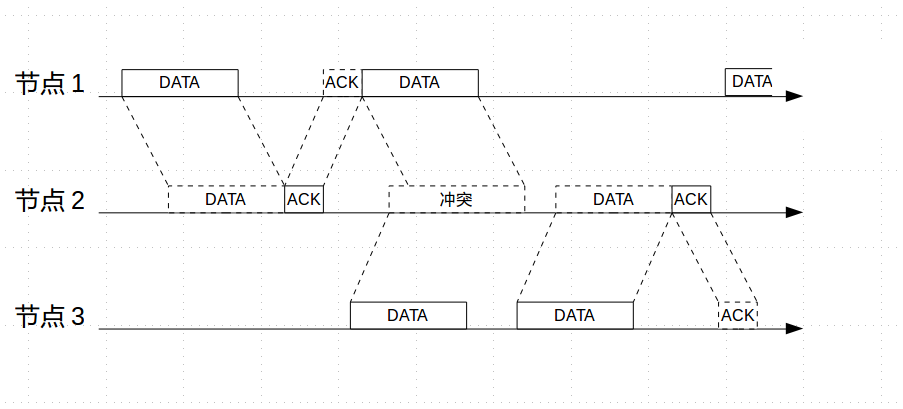
\includegraphics[scale=0.4]{figures/aloha.png}
	\caption{
		UWALOHA协议流程
	}
	\label{fig2}
\end{figure}

\subsection{性能分析}
UWALHOHA协议数据发送成功指的是在t时刻,有且只有一个节点发送的数据到达,并且没有与其他数据产生碰撞的场景。这意味着如果一个数据要经过$\Delta t$时间传播,那么它不可以在$t-\Delta t$时间发送\cite{vieira2006analysis}。

假设节点在t时刻发送数据的概率为$p$,其他$n-1$个节点不发送数据的概率为$p-1$,信道传输的成功概率为:
\begin{equation}
P_S=p(1-p)^{n-1}   0\le p\le 1
\end{equation}
最优传输成功率为
\begin{equation}
\lim\limits_{n\to+\infty} (1-\frac{1}{n})^{n-1}=\frac{1}{e}
\end{equation}
\section{SFAMA}
\subsection{协议原理}
如图\ref{fig3},在SFAMA\cite{molins2007slotted}中,当一个节点想要进行一次数据交互时,它会等待到下一个时隙时间开始传送RTS帧。目标节点和其他邻居节点会在当前时隙内接收到RTS帧。目标节点在下一个时隙开始时发送CTS帧,CTS帧会被源节点和目标节点的邻居节点接收到。源节点接收到CTS帧后,在下一个时隙时间传送DATA帧,其他邻居节点接收到CTS帧后进行退避。目标节点接收到全部数据后在下一个时隙时间发送ACK帧确认。

\begin{figure}[ht]
	\centering
	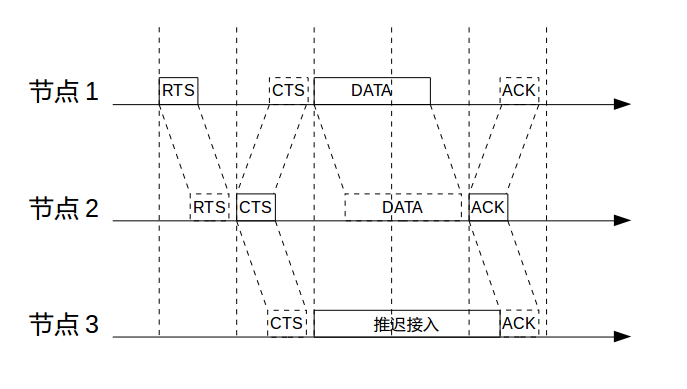
\includegraphics[scale=0.4]{figures/sf.png}
	\caption{
		SFAMA协议流程
	}
	\label{fig3}
\end{figure}

\subsection{性能分析}
假设$P_S$是信道传输的成功(无碰撞)概率。无碰撞概率指的是在节点$\omega$传输的时间间隙内没有邻居节点进行传输的概率。邻居节点可能会传输RTS帧或者还没有被接收的CTS帧进而引起碰撞。

如图\ref{fig4},节点1是节点$\omega$的邻居节点,1的邻居节点中是$\omega$隐藏终端的节点用浅灰色表示了出来。如果隐藏终端在第$n-1$时隙内向节点1发送了RTS帧,节点$\omega$在第$n$时隙内向节点1发送了RTS帧,那么节点$\omega$的RTS帧和节点1要发送的CTS帧会在第$n$时隙产生冲突。

\begin{figure}[!ht]
	\centering
	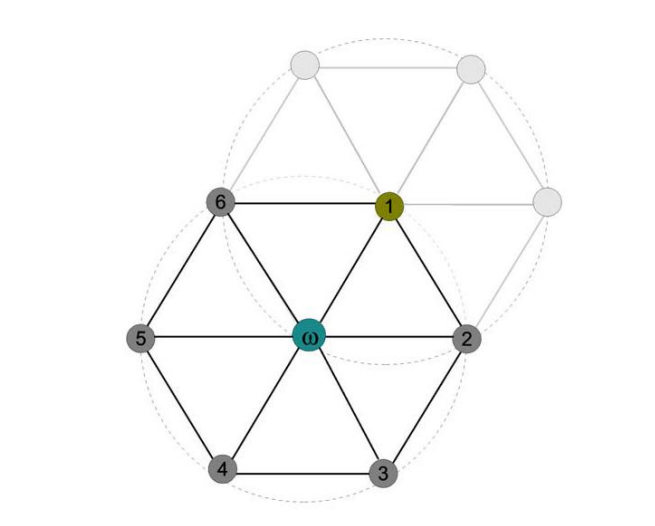
\includegraphics[scale=0.4]{figures/lay.png}
	\caption{
		网络示意图
	}
	\label{fig4}
\end{figure}

假设邻居节点数量为$N$,每一节点都以$\lambda$的速率发送数据,对于节点$\omega$的任一邻居节点,隐藏终端数量假设为Q。那么任一节点接收到特定邻居节点数据的速率是$\lambda/N$,信道传输的成功概率为
\begin{equation}
\begin{aligned}
P_S=\prod^N_1 e^{-\lambda T_{slot}}\cdot \prod^N_1 (\prod^Q_1 e^{-\frac{\lambda}{N} T_{slot}})= e^{-\lambda (N+Q) T_{slot}}
\end{aligned}
\end{equation}

一个失败周期的持续时间是两个时隙长度,第一个时隙发送RTS,第二个时隙等待接收CTS超时。所有N+1个节点以相同速率传递RTS,节点$\omega$传输RTS的速率是$\frac{1}{N+1}$,所以一个失败周期的持续时间为
\begin{equation}
\overline T_{fail}=\frac{{2T_{slot}}\cdot(1-P_S)}{N+1}
\end{equation}

一个成功周期的持续时间包括了RTS,CTS,DATA(包括由误码引起的重传时间)和ACK传输时间。假设$T_{data}$是一个DATA包传输所需要的全部时间,$T_{tot}$是一个成功周期持续时间。
\begin{equation}
T_{tot}=3T_{slot}+T_{data}
\end{equation}
\begin{equation}
\overline T_{success}=P_S \cdot T_{tot}
\end{equation}

节点的推迟接入时间包括了侦听到其他节点的CTS帧后的推迟时间和侦听到信道冲突后的推迟时间两部分,所以节点的推迟接入时间为
\begin{equation}
\overline T_{defer}=(T_{data}+T_{slot})(\frac{QP_S}{N+1}+\frac{N}{N+1}(1-P_S)) 
\end{equation}

信道平均空闲时间为
\begin{equation}
\overline I=\frac{1}{(N+1)\lambda}
\end{equation}

假设数据传输时间为$\delta$,则平均数据传输时间为
\begin{equation}
\overline U=\frac{\delta}{(N+1)P_S}
\end{equation}

根据吞吐量公式,计算得单一节点的吞吐量$(S)$为
\begin{equation}
\begin{aligned}
S&=\frac{\overline U}{\overline B+\overline I}=\frac{\overline U}{\overline T_{success}+\overline T_{fail}+\overline T_{defer}+\overline I}\\
&=\frac{\delta P_s}{(n+1)P_S T{tot}+2T_{slot}+(T_{data}+T_{slot})(QP_S+N(1-P_S))+\frac{1}{\lambda}}
\end{aligned}
\end{equation}

\endinput
\chapter{MAPA-CSMA协议设计}
MAPA-CSMA(Mobile-node Accssibility and Playload Adaptivity based CSMA)协议是根据水声网络数据采集的需求,针对有移动节点接入的单跳网络场景设计的协议。协议的基本流程参照了802.11协议,基于带有RTS/CTS模式的CSMA/CA机制,同时采用二进制退避算法计算随机退避的时间。在此基础上,考虑到移动节点的接入,加入了BCT包来通知固定节点开始发送数据。同时,随着网络负载的增加,RTS/CTS握手带来的竞争开销较大。因此,根据负载情况的不同,可以采取不同的数据包传输流程,即在较大网络负载时,一次RTS/CTS握手后发送节点传输两个数据包,目标节点在接收到第二个数据包后再进行ACK应答。

\section {基本原理介绍}
\subsection{RTS/CTS模式}
RTS/CTS模式是通过控制包预约信道来减少数据包碰撞,即用短包的碰撞代替长数据包的碰撞。发送节点准备发送数据时,首先侦听DIFS时间,如果信道空闲则开始发送RTS帧预约信道。RTS帧中包括了源节点地址,目标节点地址和本次通讯需要的最大持续时间。目标节点接收到RTS后,侦听SIFS时间后发送CTS帧进行响应。CTS帧中同样包括了源节点地址,目标节点地址和本次通讯需要的最大持续时间。非目标节点的其他节点在接收到RTS、CTS帧后,按照最大持续时间设置NAV(Network Allocation Vector 网络分配矢量),进行退避。源节点接收到CTS后,侦听SIFS时间后发送DATA帧。目标节点接收到数据包后,侦听SIFS时间后发送ACK包响应。其他节点接收到ACK包后停止退避。
\begin{figure}[ht]
	\centering
	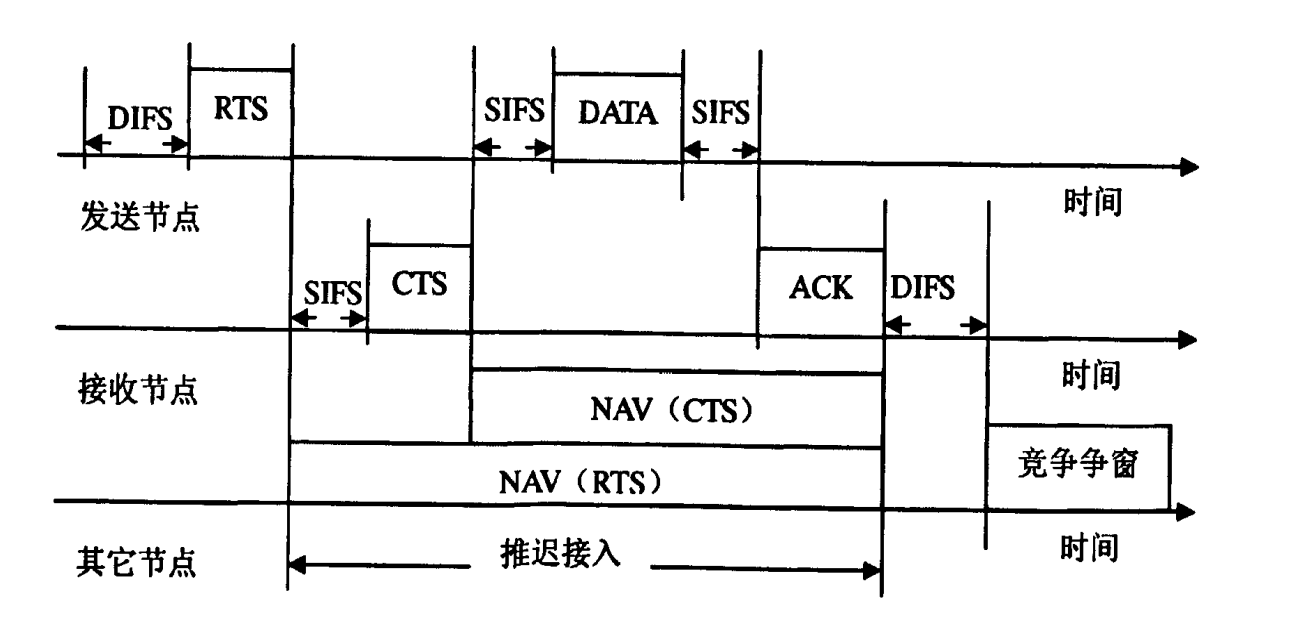
\includegraphics[scale=0.2]{figures/RC.png}
	\caption{
		RTS/CTS工作模式
	}
	\label{fig:example}
\end{figure}
\subsection{二进制退避算法}
具体算法描述如下:当一个节点要向信道发送数据时,首先侦听信道状态,若信道空闲且空闲时间达到一个DIFS时,节点立即进行数据发送,否则,即节点侦听到信道状态为“忙“,此时节点会一直侦听下去,直至侦听到节点空闲一段DIFS时间后,根据退避算法产生一个退避时间值存入退避计时器,如果此时退避计时器里面已经有了退避时间值,那么就不将新产生的退避时间值存入退避计时器,然后进行退避,以避免和其它节点发生冲突。退避时间值是退避时隙(Slot Time)的整数倍,退避时隙(Slot Time)是按物理层特性产生的值。节点在选好退避时间值后,如果信道在其退避期间一直空闲,那么节点会在一个完整的退避时隙后将退避时隙数减1,如果信道一直空闲到退避时隙数减到O时,那么节点就发送数据,否则,即退避过程中又侦听到“忙”,则进行冻结退避计时器,停止退避,直至再次侦听到一段DIFS时间信道空闲后,再次启动退避计数器进行退避(退避时间值从上次退避后的值开始计算)。
\begin{figure}[ht]
	\centering
	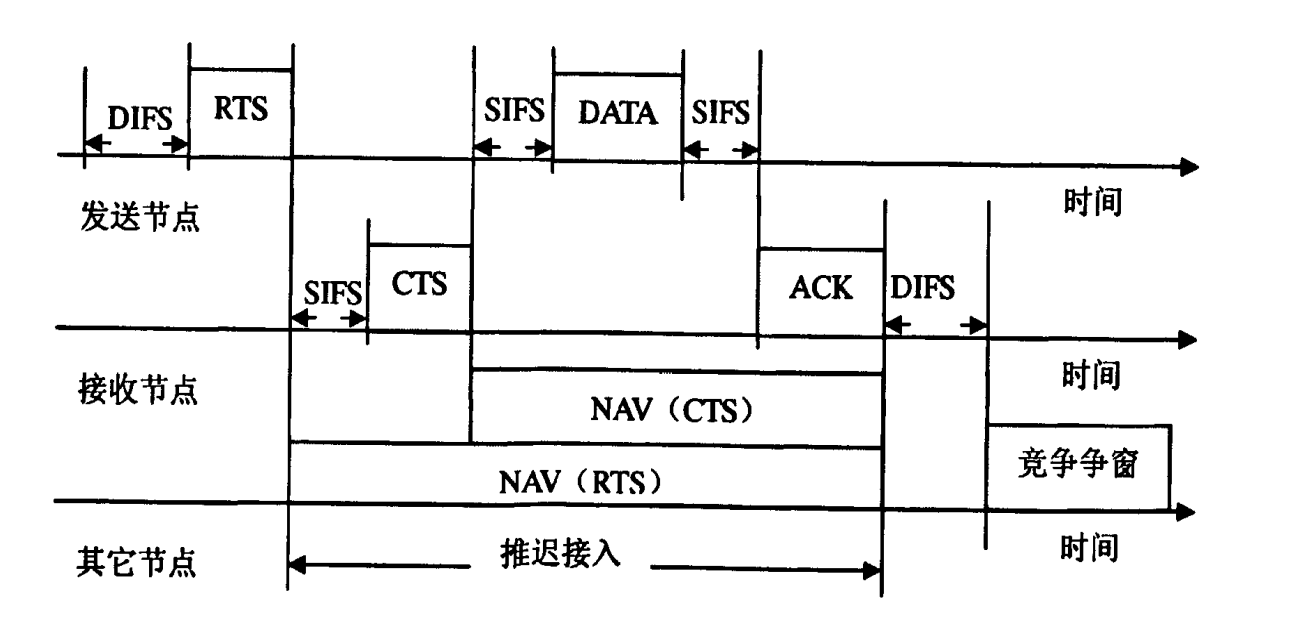
\includegraphics[scale=0.2]{figures/RC.png}
	\caption{
		RTS/CTS工作模式
	}
	\label{fig:example}
\end{figure}
\subsection{时隙和帧间间隔}
时隙(SlotTime)是指的一个时间片段,节点竞争接入信道之前需要经过相应的随机退避过程,退避过程就是由很多个时隙所组成的。参考802.11协议,时隙定义为
\begin{equation}
\begin{aligned}
SlotTime=&CCATime\mbox{(信道监测时间)}+RxTxTurnaroundTim\mbox{(发送接收)}\\&\mbox{(转换时间)}+PropagationTime\mbox{(传播延迟)}+MACProcessing\\&Delay\mbox{(MAC层处理延迟)}
\end{aligned}
\end{equation}

短帧间间隔SIFS(Short Interfram Space)是最短的时间区段,用来间隔一次对话中的帧,如响应帧(CTS/ACK)和相邻的DATA帧等。在帧交换的两次传输之间使用最短间隔,可以防止其它正在等待信道的节点试图使用信道。参考802.11协议,SIFS定义为
\begin{equation}
\begin{aligned}
SIFSTime=&RXRFDelay\mbox{(射频延迟)}+RXPLCPDelay\mbox{(物理层头部接收)}\\&\mbox{(延迟)}+MACProcessingDelay\mbox{(MAC层处理延迟)}+ RxTx\\&TurnaroundTime\mbox{(发送接收转换时间)}
\end{aligned}
\end{equation}

分布协调功能帧间间隔DIFS(DCF Interframe Space)用于节点开始发送数据之前监测信道否空闲。如果信道已经空闲,则节点仍需等待DIFS段时间才开始发送数据;而如果在DIFS时间段内任一时刻信道被监测为忙,则节点不得不推迟它的数据发送。DIFS定义为
\begin{equation}
DIFS=SIFS+(2*SlotTime)
\end{equation}

在水声信道环境中,由于传播时延导致时隙时间过长,进而导致DIFS和随机退避时间过长,即数据传输时空闲时间过长,影响了协议的整体性能。减小时隙时间可以减小空闲时间占比,但同时也会带来包冲突概率的增加。综合这两方面的影响,最后将时隙时间设定为0.5s,SIFS设定为0.5s。
\section {移动节点接入离开机制}
通过引入BCT包控制移动节点的接入和离开,其中包括了源节点地址,目标节点地址和网络负载情况。移动节点以$\frac{1}{T_{interval}}$速率定时发送广播包BCT,开始向最近的移动节点发送CBR数据流。如果固定节点在$2*T_{interval}$时间内没有接收到广播包,则停止发送CBR数据流。
\begin{figure}[ht]
	\centering
	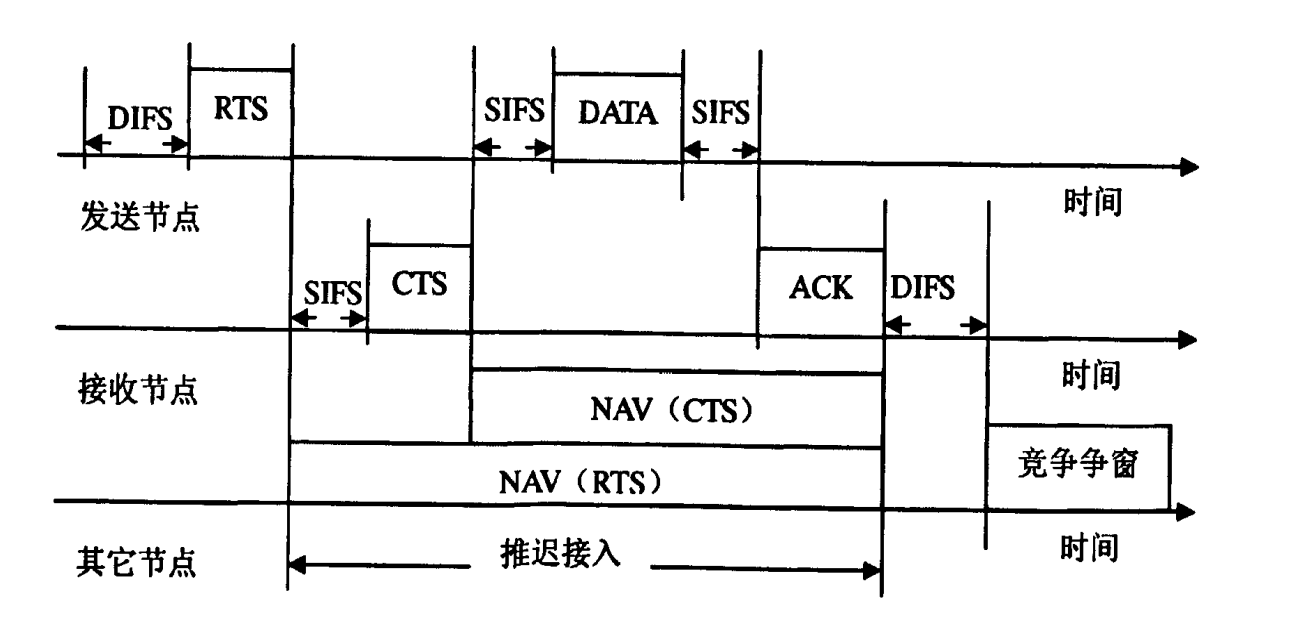
\includegraphics[scale=0.2]{figures/RC.png}
	\caption{
		移动节点接入离开机制
	}
	\label{fig:example}
\end{figure}
BCT包的发送接收不影响正在进行的一轮传输。例如在发送节点接收到CTS还未发送DATA包时接收到了BCT包,发送节点的状态仍为MAC\_CTS,在接收完BCT包后,继续发送DATA包。

HASH表

\section {数据包重传机制}
考虑到减小时隙时间导致载波侦听时间不够充分,包冲突概率增加,以及BCT包的引入带来的包冲突可能性这两个方面,加入了数据包重传机制。在802.11协议中,源节点发送了DATA包但没有收到ACK确认包的情况下,会在发送函数定时器超时后重新开始一轮新的数据传输,经过退避时间和DIFS时间倒计时后再发送RTS。这个重传流程在包冲突概率较大的情况下开销过大,影响传输性能。

因此,在发送DATA包超时后立即重传DATA包是一个可行的解决方法。同时,需要修改其他节点的推迟接入时间,在原推迟时间的基础上加上timeout(DATA包一次发送超时时间)、SIFS、txtime(传输时间)和MaxPropagationDelay(最大传播时延)。

\begin{figure}[ht]
	\centering
	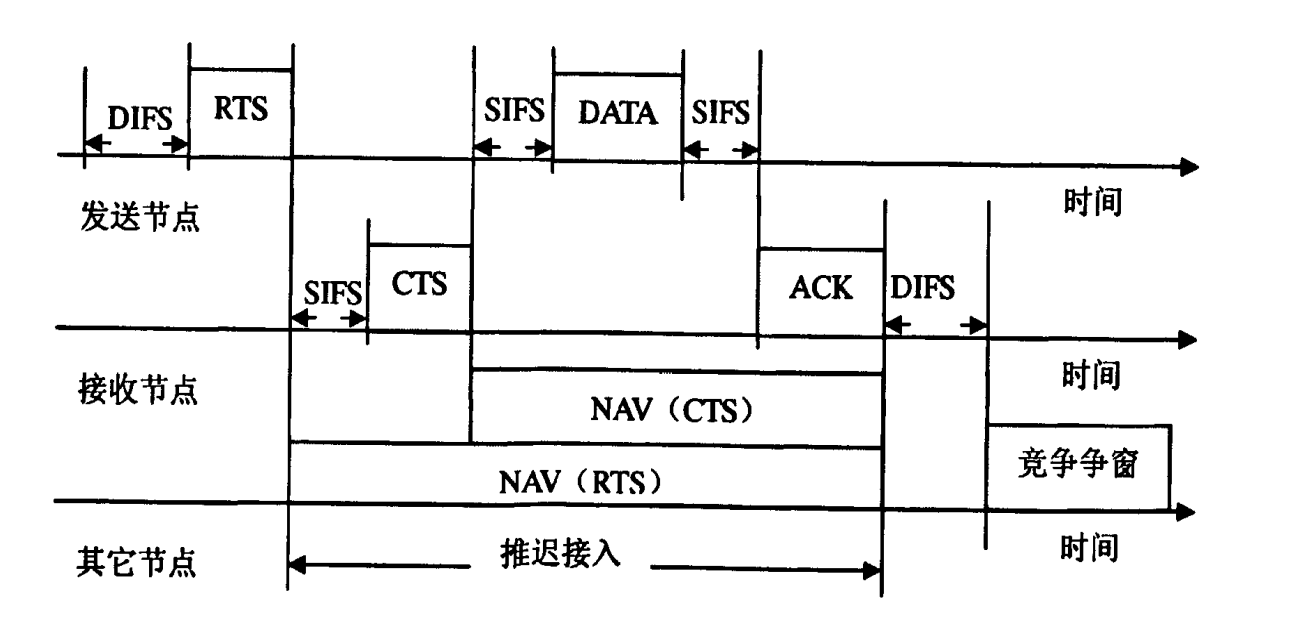
\includegraphics[scale=0.2]{figures/RC.png}
	\caption{
	     数据包一次传输超时情况下的数据包重传流程
	}
	\label{fig:example}
\end{figure}

\section {基于负载变化的数据包发送机制}
网络负载较大时,数据包的RTS/CTS握手机制带来的控制开销较大,对于不同的网络负载情形,可以采用不同的数据包传输机制。在高负载的情况下,发送节点可以在一次RTS/CTS握手后发送两个DATA包,两个DATA包间间隔SIFS,接收节点在接收到第二个DATA包后发送ACK信号。低负载的情况下,仍然采用原来的流程。

由于数据包传输机制的改变,节点的推迟接入时间和发送超时时间会有不同。可以通过在BCT包中增加一位数据位标志网络的负载情况,固定节点在接收到BCT广播后更改自己的数据传输模式。
\begin{figure}[ht]
	\centering
	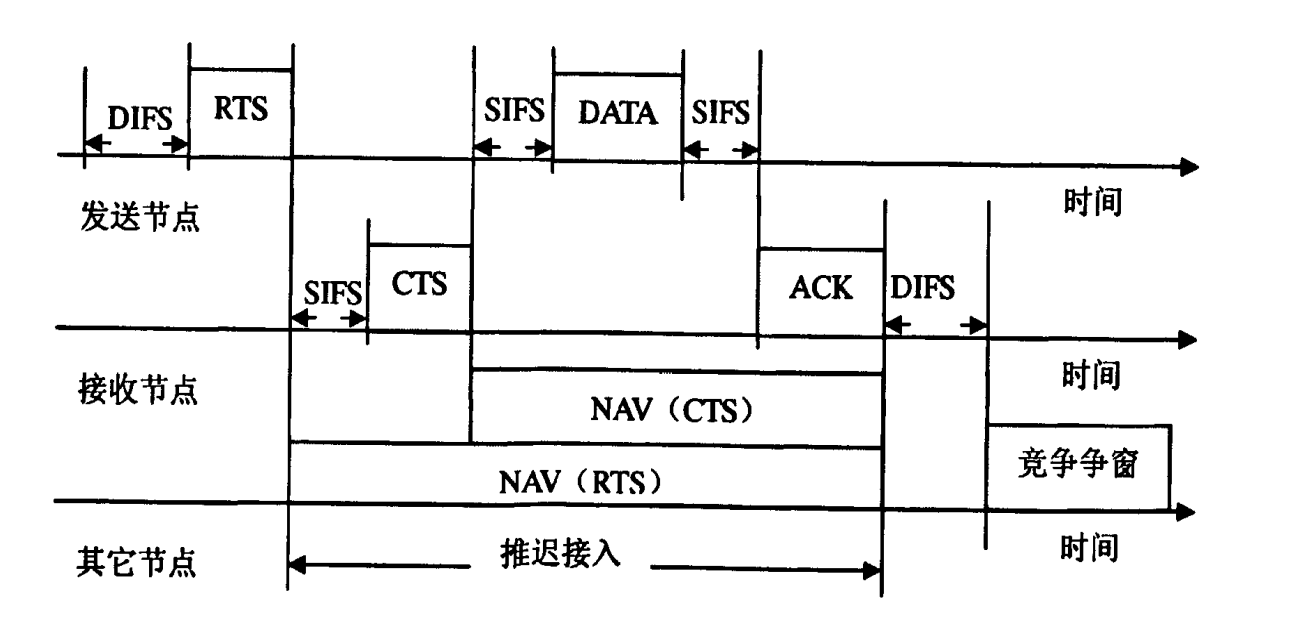
\includegraphics[scale=0.2]{figures/RC.png}
	\caption{
		高负载情况下的数据传输流程
	}
	\label{fig:example}
\end{figure}



\endinput
\chapter{协议实现和性能分析}
\section {协议实现}
\subsection{协议流程}
%    \begin{algorithm}  
%    	\caption{Calculate $y = x^n$}   
%    	\label{alg1}  
%   	\begin{algorithmic} 	 
%    		\REQUIRE $n \geq 0 \vee x \neq 0$   
%    		\ENSURE $y = x^n$   
%    		\STATE $y \Leftarrow 1$   
%    		\IF{$n < 0$}   
%    		\STATE $X \Leftarrow 1 / x$   
%   		\STATE $N \Leftarrow -n$   
%    		\ELSE   
%    		\STATE $X \Leftarrow x$   
%    		\STATE $N \Leftarrow n$  
%    		\ENDIF   
%    		\WHILE{$N \neq 0$}   
%   		\IF{$N$ is even}   
%    		\STATE $X \Leftarrow X \times X$   
%    		\STATE $N \Leftarrow N / 2$   
%    		\ELSE[$N$ is odd]   
%    		\STATE $y \Leftarrow y \times X$   
%    		\STATE $N \Leftarrow N - 1$   
%    		\ENDIF   
%    		\ENDWHILE  
%    	\end{algorithmic}  
%    \end{algorithm}  

状态转移图
RXSTATE

 \begin{figure}[!ht]
 	\centering
 	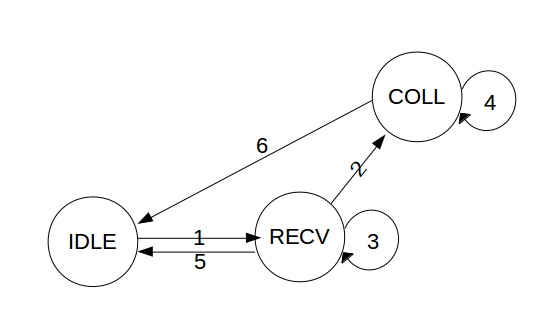
\includegraphics[scale=0.5]{figures/rxstate.png}
 	\caption{
 		rxstate
 	}
 	\label{fig:example}
 \end{figure}
 
\begin{table}[!ht]
	\centering
\begin{tabular}{c c c}
	\hline  % 在表格最上方绘制横线
	 &状态转移条件&执行的操作\\
	\hline  % 在表格最上方绘制横线
	1&节点空闲状态下侦听到包 & 接收包到pktRx\_\\
	2&节点接收状态下收到其他包,不满足接收条件&节点状态置为冲突状态,清空pktRx\_\\
	3&在接收状态下收到其他包,满足接收条件&节点设置NAV推迟接入,接收新包到pktRx\_,接收完毕后节点状态置为空闲\\
	4&在冲突状态下收到其他包,不满足接收条件&节点状态仍为冲突状态,清空pktRx\_\\
	5&在接收状态下接收完到达包以后&节点状态置为空闲\\	
	6&在冲突状态下收到其他包,满足接收条件&节点设置NAV推迟接入,接收新包到pktRx\_,接收完毕后节点状态置为空闲\\
	\hline
\end{tabular}
\end{table}

txstate
 \begin{figure}[!ht]
 	\centering
 	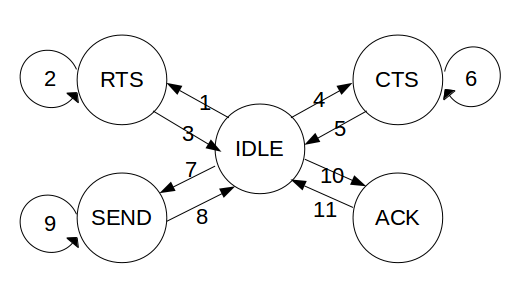
\includegraphics[scale=0.5]{figures/txstate.png}
 	\caption{
 		txstate
 	}
 	\label{fig:example}
 \end{figure}
 
\begin{table}[!ht]
	\centering
	\begin{tabular}{c c c}
		\hline  % 在表格最上方绘制横线
		&状态转移条件&执行的操作\\
		\hline  % 在表格最上方绘制横线
		1&节点准备开始一次数据传输 &准备pktRTS\_、pktTx\_,节点状态置为RTS\\
		2&RTS状态下接收到RTS、DATA、ACK、BCT包&节点状态不变,丢弃除BCT以外的接收到的包\\
		3&RTS状态下接收到CTS包清空pktRTS\_后或RTS状态超时&发送状态置为空闲,开始下一次发送\\
		4&接收完RTS包,发送状态空闲&准备pktCTRL\_,发送状态置为CTS,发送CTS包\\
		5&CTS状态下接收到DATA包清空pktCTRL\_后或CTS状态超时&发送状态置为空闲,开始下一次发送\\
		6&CTS状态下接收到RTS、CTS、ACK、BCT包&节点状态不变,丢弃除BCT以外的接收到的包\\
		7&接收完CTS包,发送状态空闲&准备pktTx\_发送状态置为MAC\_SEND,发送DATA包\\
		8&SEND状态下接收到ACK包清空pktTx\_后或SEND状态超时&发送状态置为空闲,开始下一次发送\\
		9&SEND状态下接收到RTS、CTS、DATA、BCT包&节点状态不变,丢弃除BCT以外的接收到的包\\
		10&接收完DATA包,发送状态空闲&准备pktCTRL\_,发送状态置为ACK,发送ACK包\\
		11&ACK发送完成&发送状态置为空闲,开始下一次发送\\
		\hline
	\end{tabular}
\end{table}

\subsection{帧格式}
BCT\\
\begin{tabular}{|c|c|c|}% 通过添加 | 来表示是否需要绘制竖线
	\hline  % 在表格最上方绘制横线
	名称&功能描述&字段位数(字节)\\
	\hline  %在第一行和第二行之间绘制横线
	Frame Control& &2\\
	\hline % 在表格最下方绘制横线
	Duration&持续时间&2\\
	\hline
	Receiver Address&接收节点地址&6\\
	\hline
	Transmitter Address&发送节点地址&6\\
	\hline
	网络负载情况&分为高低两种&1\\
	\hline
	Transmitter Address&发送节点地址&1\\
	\hline
	FCS&帧校验序列,用来检查所收到帧的完整性&4\\
	\hline
\end{tabular}

RTS/CTS/ACK\\
\begin{tabular}{|c|c|c|}% 通过添加 | 来表示是否需要绘制竖线
	\hline  % 在表格最上方绘制横线
	名称&功能描述&字段位数(字节)\\
	\hline  %在第一行和第二行之间绘制横线
	Frame Control&帧的subtype位,1011代表RTS,1100 CTS,1101 ACK&2\\
	\hline % 在表格最下方绘制横线
	Duration&持续时间&2\\
	\hline
	Receiver Address&接收节点地址&6\\
	\hline
	Transmitter Address&发送端地址,RTS帧的发送端的地址。&6\\
	\hline
	FCS&帧校验序列,用来检查所收到帧的完整性&4\\
	\hline
\end{tabular}

DATA\\
\begin{tabular}{|c|c|c|}% 通过添加 | 来表示是否需要绘制竖线
	\hline  % 在表格最上方绘制横线
	名称&功能描述&字段位数(字节)\\
	\hline  %在第一行和第二行之间绘制横线
	Frame Control&  &2\\
	\hline % 在表格最下方绘制横线
	持续时间(Duration ID)&用来记载网络分配矢量(Network Allocation Vector,简称NAV)&2\\
	\hline
	目的地址&最后的接收端,即负责将帧交付上层协议处理的工作站&6\\
	\hline
	源地址&传送的来源&6\\
	\hline
	接收端地址&负责处理该帧的无线工作站&6\\
	\hline
	顺序控制字段(Seq-Ctl)&用来重组帧片段以及丢弃重复帧&2\\	
	\hline
	发送端地址&将帧传送至无线媒介的无线接口&6\\
	\hline
	FCS&帧校验序列,用来检查所收到帧的完整性&4\\
	\hline
\end{tabular}

\section {性能分析}
按照流量模型,信道时间可以划分为信道繁忙时间和信道空闲时间,信道的平均利用率等于发送有效数据的时间和总时间的比值。
\begin{equation}
S=\frac{\overline U}{\overline O+\overline I}
\end{equation}

其中,$\overline U$表示发送有效数据传输时间的期望值,$\overline O$表示信道繁忙时间的期望值,$\overline I$表示信道空闲时间的期望值。
	
\subsection {低负载模式}
在MAPA-CSMA协议中,隐藏终端传输的RTS帧和移动节点定时发送的BCT帧会引起冲突。对于第一种情况,移动节点$\alpha$是固定节点$\omega$和固定节点$\beta$的邻居节点,节点$\beta$是节点$\omega$的隐藏终端。节点$\alpha$在和节点$\omega$进行数据交互的过程中,节点$\beta$发送的RTS帧可能会使得节点$\alpha$接收$\omega$的RTS帧和DATA帧产生碰撞。第二种情况中,除$\alpha$以外的其他邻居移动节点发送的BCT帧会对$\omega$接收CTS和ACK帧产生碰撞。

假设$P_S$是信道传输的成功概率,也就是在节点$\omega$数据交互周期内没有发生包碰撞的概率。节点$\omega$的邻居节点数量为M。$\omega$邻居移动节点的隐藏终端数量假设为Q,其中固定终端数量为$Q_s$,移动终端为$Q_m$,。任一隐藏终端以$\lambda/N$的速率向移动节点$\alpha$发送RTS包。移动节点$\alpha$以$\mu$的速率定时发送BCT包。

随机退避时间$CW_{min}=W$,$CW_{max}=2_r W$,在第i阶段的退避过程中可随机选择的退避时间为:
\begin{equation}
W_i=2^iW_i \ \ \ i\in(0,r)
\end{equation}
为了简化模型,只考虑第一阶段的退避过程,可选择的退避时间为$(0,W)$。

信道传输成功概率为:
\begin{equation}
P_S=\lambda(1-\lambda)^{M+Q_s}(1-\mu)^{Q_m}
\end{equation}

节点推迟接入包括接收到邻居节点的RTS帧和接收到邻居节点响应隐藏终端RTS帧而发送的CTS帧,因收到RTS帧推迟接入的概率为
\begin{equation}
 P_{Rdefer}=(1-\lambda)\lambda M
\end{equation}
因收到CTS帧推迟接入的概率为
\begin{equation}
 P_{Cdefer}=(1-\lambda)\lambda Q
\end{equation}

一个失败周期的持续时间是等待发送RTS帧的时间和发送RTS未收到CTS回复的超时时间,设最大传输时延为$\tau$
\begin{equation}
\begin{aligned}
T_{fail}&=T_{DIFS}+\overline W+Tout_{RTS}\\
&=T_{DIFS}+\overline W+T_{RTS}+2\tau+T_{SIFS}+T_{CTS}
\end{aligned}
\end{equation}

一个成功周期的持续时间包括了RTS,CTS,DATA和ACK的一整个流程。
\begin{equation}
T_{suc}=T_{DIFS}+\overline W+T_{RTS}+T_{CTS}+T_{DATA}+T_{ACK}+4\tau+3T_{SIFS}
\end{equation}

因收到RTS帧推迟接入的时间为
\begin{equation}
T_{Rdefer}=T_{CTS}+T_{DATA}+T_{ACK}+3\tau+3T_{SIFS}
\end{equation}

因收到CTS帧推迟接入的时间为
\begin{equation}
T_{Rdefer}=T_{DATA}+T_{ACK}+2\tau+2T_{SIFS}
\end{equation}

\begin{equation}
\overline B=T_{suc}P_S+T_{fail}(\lambda-P_S )+ T_{Cdefer}P_{Cdefer}+T_{Rdefer}P_{Rdefer}
\end{equation}

信道空闲时间为:
\begin{equation}
\overline I=\left\{
\begin{aligned}
1-B \ \ \ \ \ \ \ \ B<1\\
0\ \ \ \ \ \ \ \    B\ge 1
\end{aligned}
\right.
\end{equation}

根据吞吐量公式,计算得单一节点的吞吐量$(S)$为
\begin{equation}
\begin{aligned}
S&=\frac{\overline U}{\overline B+\overline I}\\&=\frac{T_{DATA}}{ T_{suc}P_S+T_{fail}(\lambda-P_S )+ T_{Cdefer}P_{Cdefer}+T_{Rdefer}P_{Rdefer}+\overline I}
\end{aligned}
\end{equation}

\subsection {高负载模式}

信道传输成功概率为:
\begin{equation}
P_S=\frac{\lambda}{2}(1-\frac{\lambda}{2})^{M+Q_s}(1-\mu)^{Q_m}
\end{equation}

节点推迟接入包括接收到邻居节点的RTS帧和接收到邻居节点响应隐藏终端RTS帧而发送的CTS帧,因收到RTS帧推迟接入的概率为
\begin{equation}
P_{Rdefer}=(1-\frac{\lambda}{2})\cdot\frac{\lambda}{2} M
\end{equation}
因收到CTS帧推迟接入的概率为
\begin{equation}
P_{Cdefer}=(1-\frac{\lambda}{2})\cdot\frac{\lambda}{2} Q
\end{equation}

一个失败周期的持续时间是等待发送RTS帧的时间和发送RTS未收到CTS回复的超时时间,设最大传输时延为$\tau$
\begin{equation}
\begin{aligned}
T_{fail}&=T_{DIFS}+\overline W+Tout_{RTS}\\
&=T_{DIFS}+\overline W+T_{RTS}+2\tau+T_{SIFS}+T_{CTS}
\end{aligned}
\end{equation}

一个成功周期的持续时间包括了RTS,CTS,2DATA和ACK的一整个流程。
\begin{equation}
T_{suc}=T_{DIFS}+\overline W+T_{RTS}+T_{CTS}+2T_{DATA}+T_{ACK}+4\tau+4T_{SIFS}
\end{equation}

因收到RTS帧推迟接入的时间为
\begin{equation}
T_{Rdefer}=T_{CTS}+2T_{DATA}+T_{ACK}+3\tau+4T_{SIFS}
\end{equation}

因收到CTS帧推迟接入的时间为
\begin{equation}
T_{Rdefer}=2T_{DATA}+T_{ACK}+2\tau+2T_{SIFS}
\end{equation}

信道繁忙时间为:
\begin{equation}
\overline B=T_{Cdefer}P_{Cdefer}+T_{Rdefer}P_{Rdefer}
\end{equation}

信道空闲时间为:
\begin{equation}
\overline I=\left\{
\begin{aligned}
1-B \ \ \ \ \ \ \ \ B<1\\
0\ \ \ \ \ \ \ \    B\ge 1
\end{aligned}
\right.
\end{equation}

根据吞吐量公式,计算得单一节点的吞吐量$(S)$为
\begin{equation}
\begin{aligned}
S&=\frac{\overline U}{\overline B+\overline I}\\&=\frac{2T_{DATA}}{ T_{suc}P_S+T_{fail}(\lambda-P_S )+ T_{Cdefer}P_{Cdefer}+T_{Rdefer}P_{Rdefer}+\overline I}
\end{aligned}
\end{equation}

\endinput
\chapter{水声传感网络MAC协议仿真}
\section {仿真软件介绍}
\subsection{NS2}
NS2(Network Simulator version2)是一种面向对象的网络仿真器,本质上是一个离散事件模拟器,由UC Berkeley开发而成。它本身有一个虚拟时钟,所有的仿真都由离散事件驱动的。
NS2使用C++和Otcl作为开发语言。它包含仿真事件调度器、网络组件对象库以及网络构建模型库等。事件调度器计算仿真时间,并且激活事件队列中的当前事件,执行一些相关的事件,网络组件通过传递分组来相互通信,但这并不耗费仿真时间。所有需要花费仿真时间来处理分组的网络组件都必须要使用事件调度器。它先为这个分组发出一个事件,然后等待这个事件被调度回来之后,才能做下一步的处理工作。事件调度器的另一个用处就是计时。

\subsection{Aqua-Sim}
美国康涅狄格州大学的水下无线通迅网络研究所在NS2的基础上扩展了专门用于水下环境的仿真平台Aqua-Sim\cite{xie2009aqua}。它可以十分逼真地仿真水声信道,对信号衰减和水下包碰撞的仿真十分有效。同时它也实现了一套完整的从物理层到应用层的协议栈,各层之间可以独立发展。

 \begin{figure}[!ht]
 	\centering
 	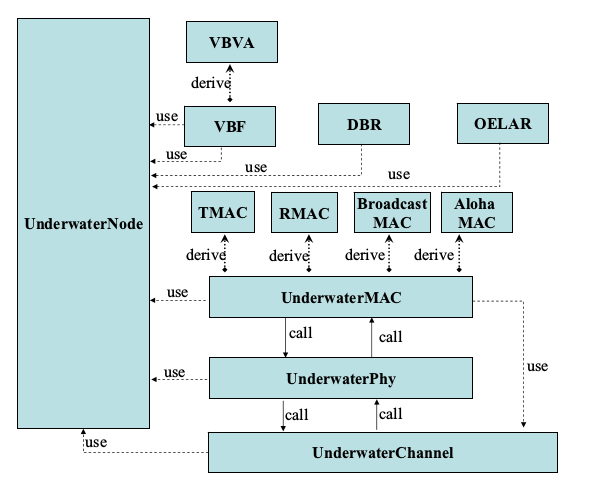
\includegraphics[scale=0.5]{figures/aq.png}
 	\caption{
 		Aqua-Sim结构
 	}
 	\label{fig:example}
 \end{figure}
\subsubsection{衰减模型}
根据传输频率$f$,距离$l$,可得吸收系数$\alpha$为\cite{xie2009aqua}
\begin{equation}
\alpha=\frac{0.11f^2}{1+f^2}+\frac{44f^2}{4100+f^2}+3.0*10^{-4}f^2+3.3*10^{-3}
\end{equation}
进而可以算出传播损失\cite{xie2009aqua}
\begin{equation}
A(l,f)=l^k\times(10^{\frac{\alpha (f)}{10}})^l
\end{equation}
根据发送功率和传播损失可以计算出接收功率的阈值。
\begin{equation}
TxThresh=\frac{Pt}{A(l,f)}
\end{equation}

\subsubsection{能量模型}
节点设置IDLE,SEND,RECV三种不同的能量状态。将节点不同状态下的功率乘以状态持续时间,可以计算出节点的能耗。仿真时调用Aqua-sim的EnergyModel类,则可以进行实时的能量追踪。

\subsubsection{碰撞模型}
节点接收数据时,如果节点正处于接收状态,计算到达数据包的能量和正在接收数据包的能量之比,和比较阈值$CPThresh$进行对比。
\begin{equation}
\begin{aligned}
&if \ \ \  \frac{Pr_{\mbox{到达}}}{Pr_{\mbox{接收}}}\  > CPThresh\\
&\ \ \ \ \ \ capture(\mbox{到达数据包});\\
&else\\
&\ \ \ \ \ \ collision(\mbox{到达数据包});
\end{aligned}
\end{equation}

\section{网络性能指标}
在处理相同数据流的情况下,判断不同MAC协议下网络性能的好坏时,主要统计四个网络数据指标,网络的平均时延、网络的平均吞吐量、网络的能耗、网络的数据包发送成功率。

(1)网络的平均时延是指数据包从源节点到达目的节点在网络中的传播时间。网络的时延=数据包的发送时延+数据包的传输时延+数据包的接收时延。 
\begin{equation}
\overline{T_{delay}}=\frac {\sum (T_{send}+T_{prop}T_{receive})}{\sum {N_{packet}}}
\end{equation}

(2)网络吞吐量表示网络成功发送的数据包数。网络的平均吞吐量定义为吞吐量主要用于衡量网络利用率和网络数据最大容量。
\begin{equation}
Throughout=\frac{Pkt_{recv} L_{data}}{T_{runtime}}
\end{equation}

(3)网络的数据包发送成功率是指网络中正确接收到的数据包数和总的发送数据包数的比值。
\begin{equation}
P_{succ}=\frac{Pkt_{send}}{Pkt_{recv}}
\end{equation}

(4)网络的平均能耗定义为网络中的所有节点在整个网络运行期间所消耗的总的能量与正确接收到的数据包数的比值。
\begin{equation}
\overline E=\frac{E_{consumed}}{Pkt_{recv}}
\end{equation}

\section {仿真实验一}
\subsection{场景设计}
场景设置仿照AUV进行数据收集的情景,进行单跳移动水声网络的仿真。图中黑色代表固定节点,红色代表移动节点,红色虚线箭头指示了移动节点的移动路径。随着移动节点的移动,网络的拓扑结构会发生动态变化。固定节点会选择合适的移动节点进行数据传输。

 \begin{figure}[!ht]
 	\centering
 	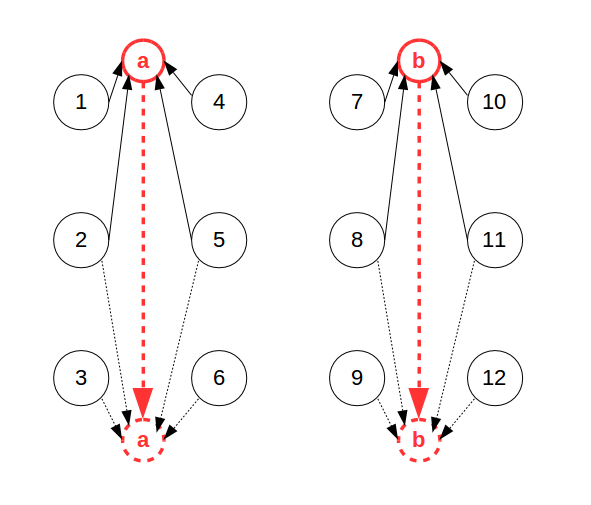
\includegraphics[scale=0.5]{figures/2scen.png}
 	\caption{
 		两移动节点场景设计
 	}
 	\label{fig:example}
 \end{figure}

节点工作参数的设置长S2CR 18/34水声通信机,参数设置如下:
\renewcommand{\arraystretch}{1.2}
\begin{table}[!htp]
	\centering
\caption{参数设置}
\begin{tabular}{m{5cm}<{\centering} m{5cm}<{\centering}}% 通过添加 | 来表示是否需要绘制竖线
	\hline  % 在表格最上方绘制横线
    参数名称& 值\\
	\hline  
	固定节点数& 12\\
	移动节点数& 2\\
	移动节点运动速度& 2.5m/s\\
	节点通信半径& 3000m\\
	相邻固定节点距离& 2000m\\
	仿真时间数& 2400s\\
	频率& 10kHz\\			
	节点传输速率& 1kbps\\
	数据包大小& 300Bytes\\
	节点发送报文功率& 30w\\				
	节点接收报文功率& 1w\\
	节点侦听报文功率& 0.2w\\
	\hline 		
\end{tabular}
\label{tab2}
\end{table}

\subsection{理论性能曲线}
按照节点的邻居节点个数和隐藏终端个数的不同,将整个仿真时间划分为不同的时间段,累计12个固定节点在所有时间段的吞吐量和,得到网络的理论吞吐量值。

仿真数据产生速率从0到0.36pkt/s(12个节点的总速率)内每0.012pkt/s的网络吞吐量,每个速率仿真十次取平均值,得到仿真吞吐量曲线。

可以看出,理论曲线与仿真曲线的走向趋势一致且误差不大,证明了理论性能曲线的准确性。
\begin{figure}[!ht]
	\centering
	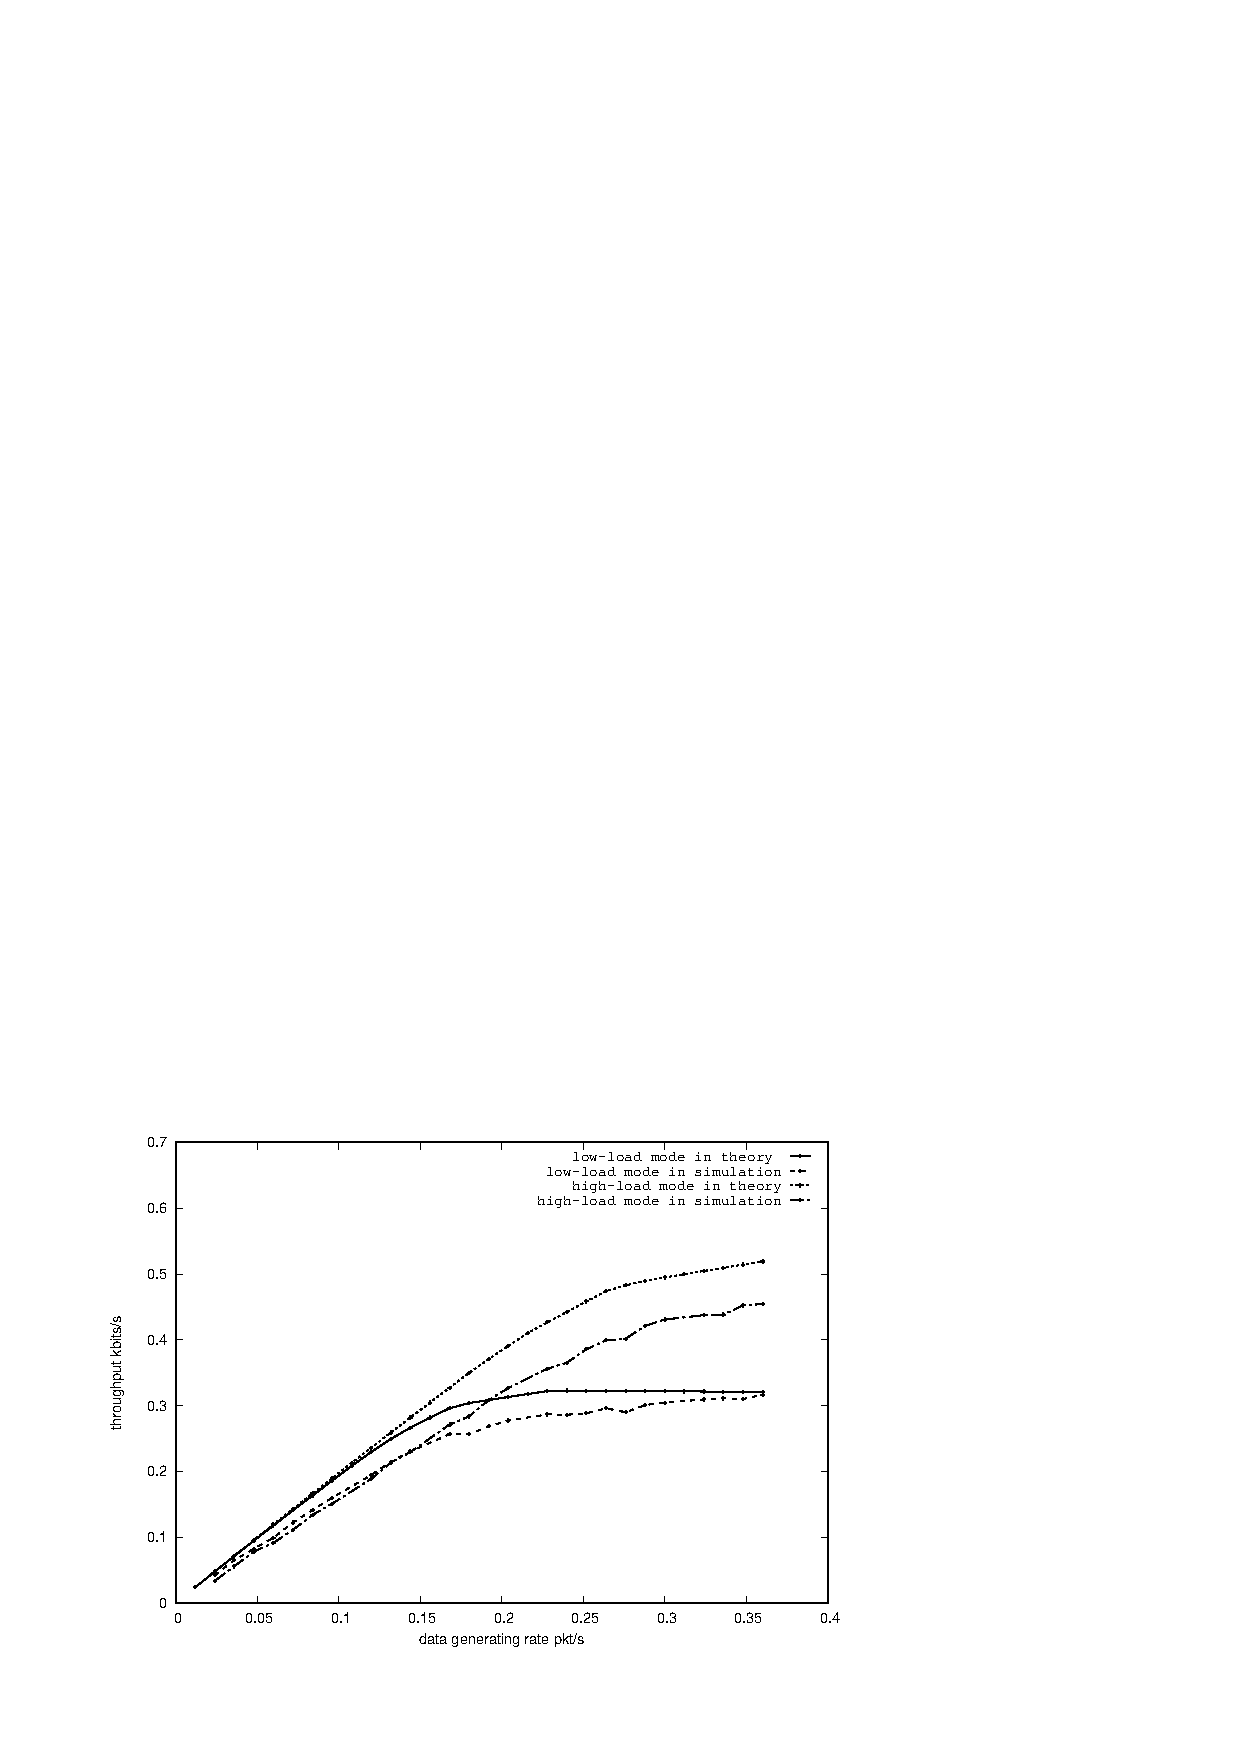
\includegraphics[scale=0.95]{figures/lilun.pdf}
	\caption{
		理论性能曲线
	}
	\label{fig:example}
\end{figure}

\subsection{结果分析}
可以看出,在网络负载较高的情况下,高负载模式协议的吞吐量远远优于低负载模式,说明握手机制在网络负载较高时引起的开销过大,影响网络性能。高负载模式的两次数据传输机制是有效的。
\begin{figure}[!ht]
	\centering
	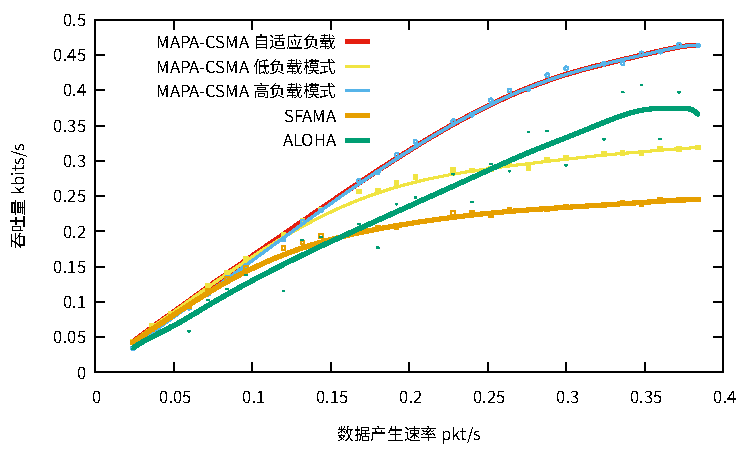
\includegraphics[scale=0.95]{figures/2nodea.pdf}
	\caption{
		吞吐量与数据产生速率关系图
	}
	\label{fig:example}
\end{figure}

由于高负载模式的两次数据传输机制需要等待第二个数据包到达才开始传输,所以在网络负载较低的情况下会引起端到端时延过大,因此自适应网络负载的数据传输机制是必要的。负载增加时,SFAMA的端到端时延会显著增加,ALOHA则对负载的变化不敏感。说明高负载网络中,握手开销极大得影响了网络性能。
\begin{figure}[!ht]
	\centering
	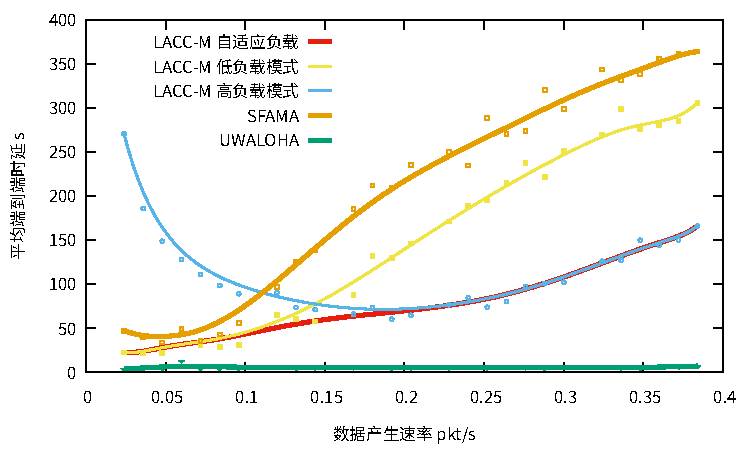
\includegraphics[scale=0.95]{figures/2nodeb.pdf}
	\caption{
		平均端到端时延与数据产生速率关系图
	}
	\label{fig:example}
\end{figure}

LACC-M协议的发送成功率显著优于SFAMA和UWALOHA协议。数据产生速率增加,即网络负载量增加对SFAMA协议的发送成功率影响较大,提出协议的改进则有效得减小了高负载下的冲突。
\begin{figure}[!ht]
	\centering
	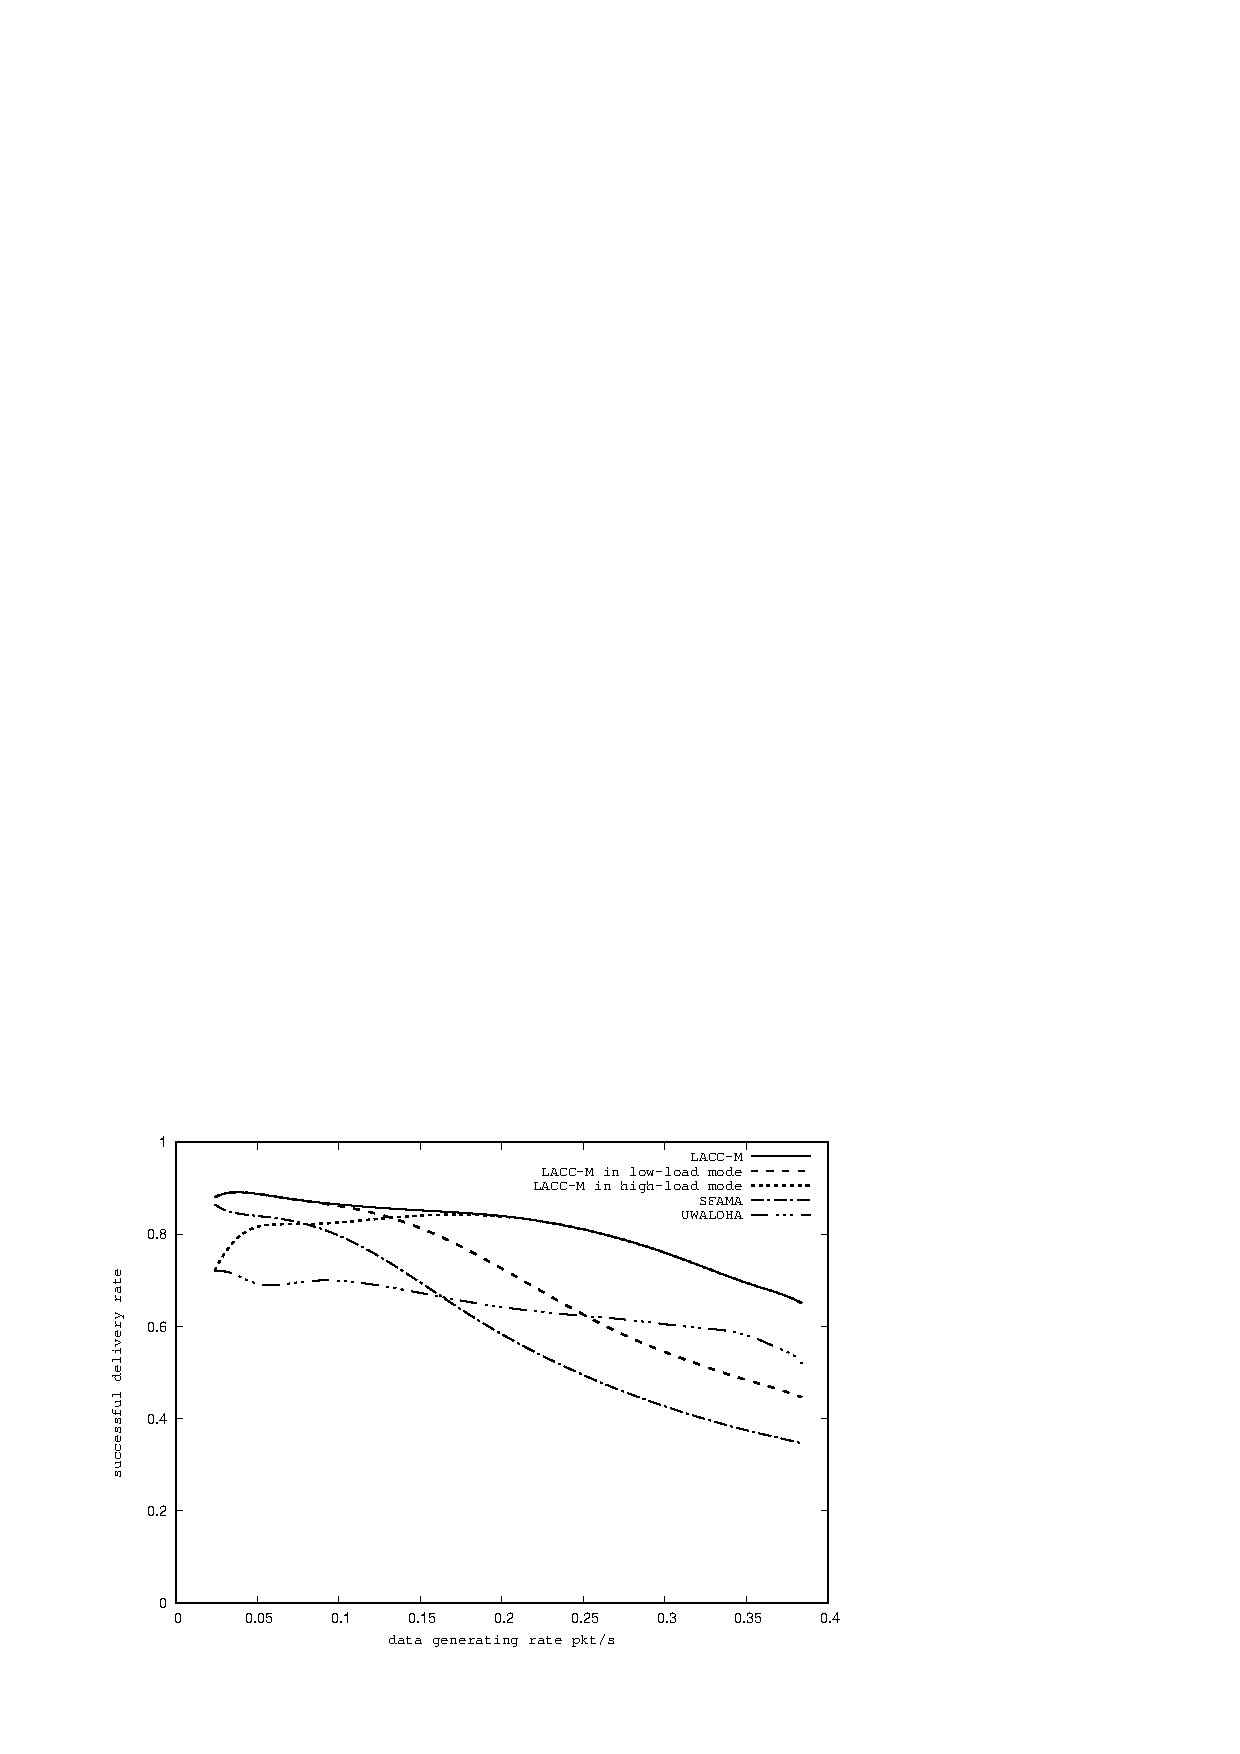
\includegraphics[scale=0.95]{figures/2nodec.pdf}
	\caption{
		发送成功率与数据产生速率关系
	}
	\label{fig:example}
\end{figure}

LACC-M协议的平均能耗在不同数据产生速率下表现都令人满意。ALOHA协议由于多次发送长数据包,所以平均能耗较高。

\begin{figure}[!ht]
	\centering
	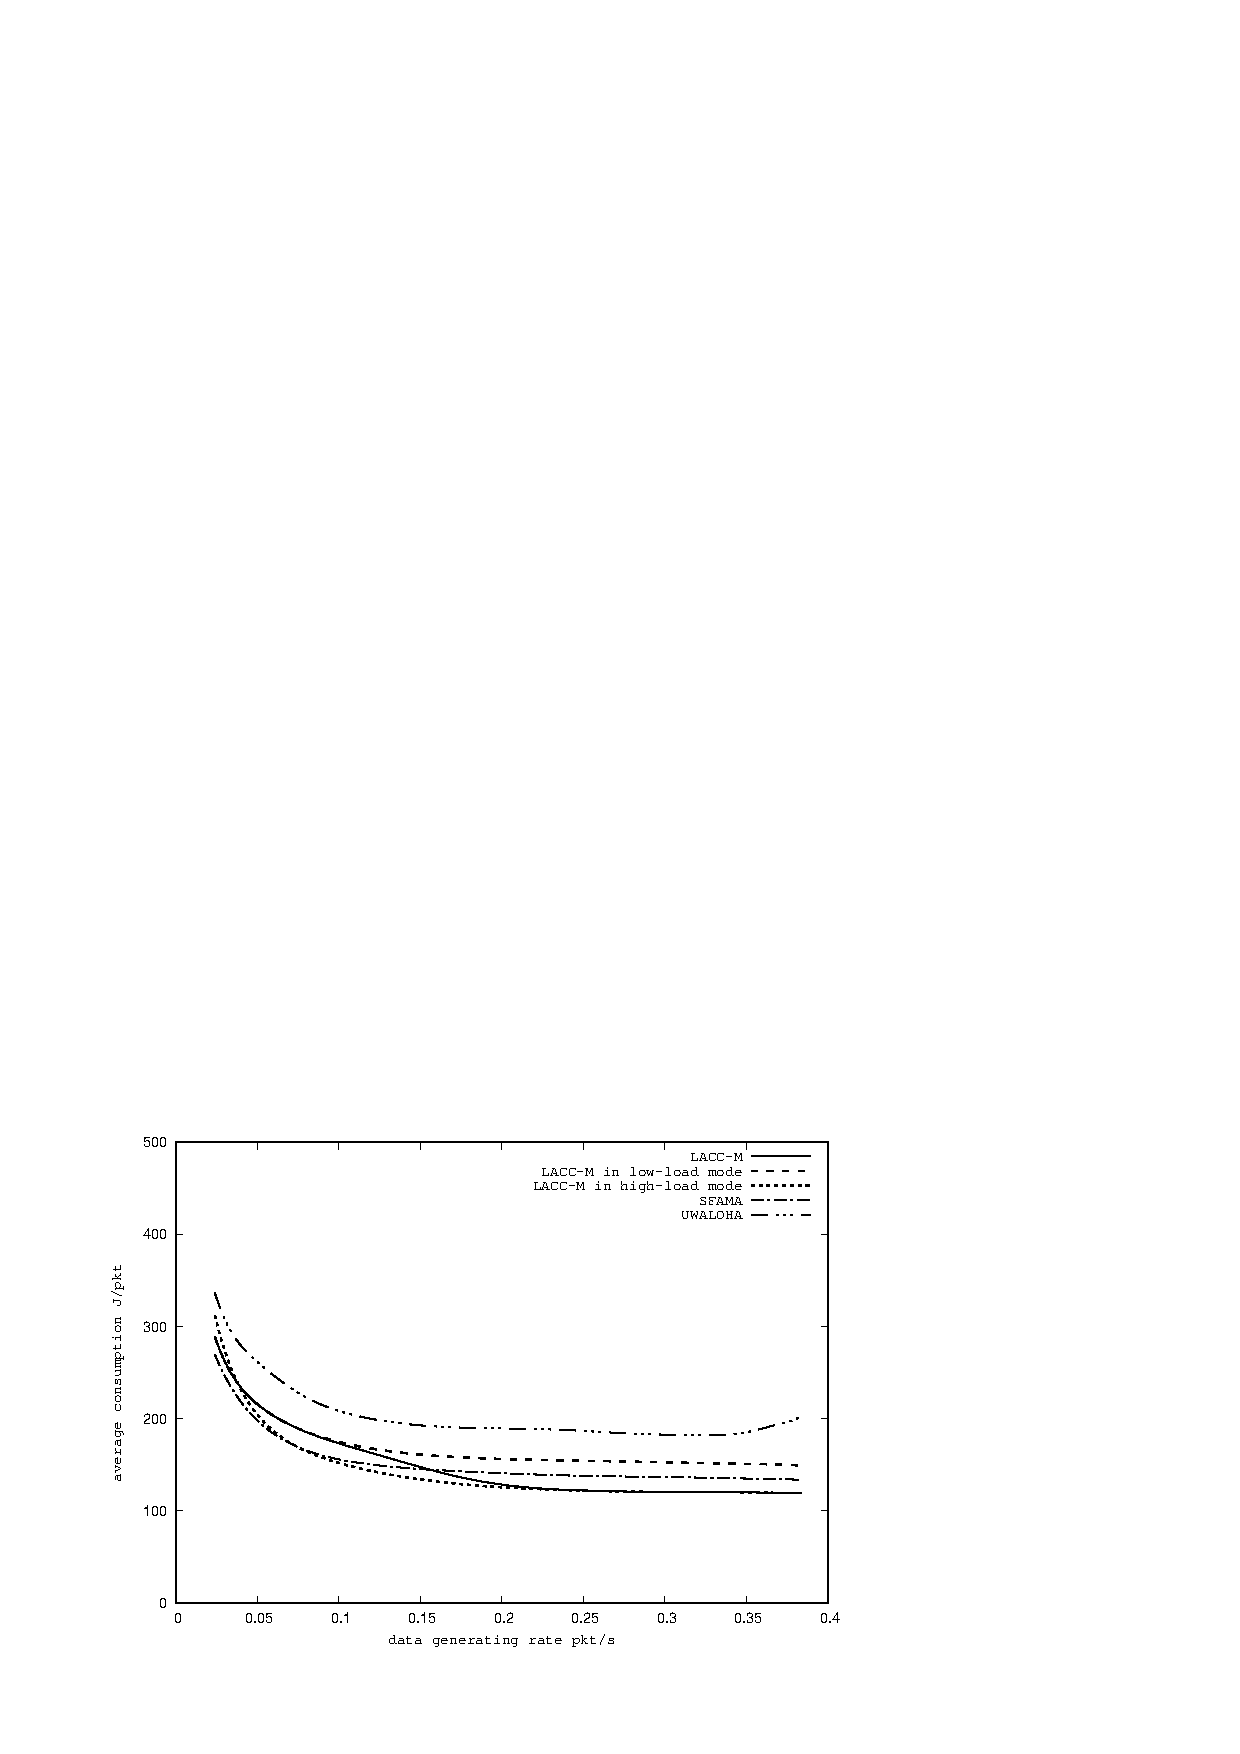
\includegraphics[scale=0.95]{figures/2noded.pdf}
	\caption{
		平均能耗与数据产生速率关系
	}
	\label{fig:example}
\end{figure}

\section {仿真实验二}
\subsection{场景设计}
考虑到固定节点通信范围内存在多个移动节点的场景,增加移动节点数量后进行了第二组仿真。仿真参数和第一组仿真相同。移动节点的移动方向与原有的两节点方向相反,由下向上移动,可以更好得提高信道的利用率。

\begin{figure}[!ht]
	\centering
	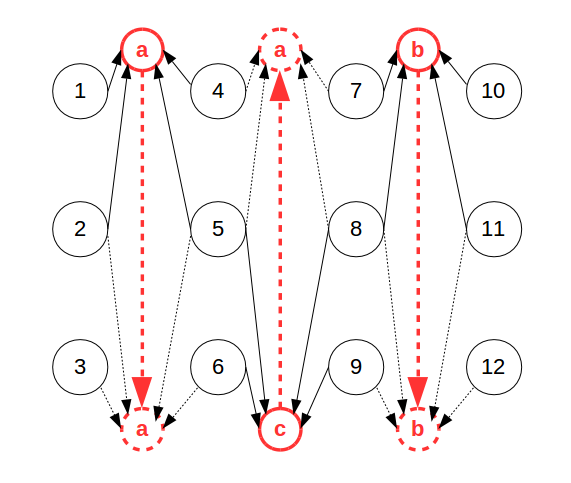
\includegraphics[scale=0.52]{figures/3scen.png}
	\caption{
		三移动节点场景设计
	}
	\label{fig:example}
\end{figure}

\subsection{结果分析}
由于多加入了移动节点,网络拓扑的动态性变高,高负载网络的吞吐量比二移动节点的网络有所下降,网络吞吐量的临界值下降。协议的吞吐量均随数据产生速率的增加而增加,整长速率逐渐放缓。

\begin{figure}[!ht]
	\centering
	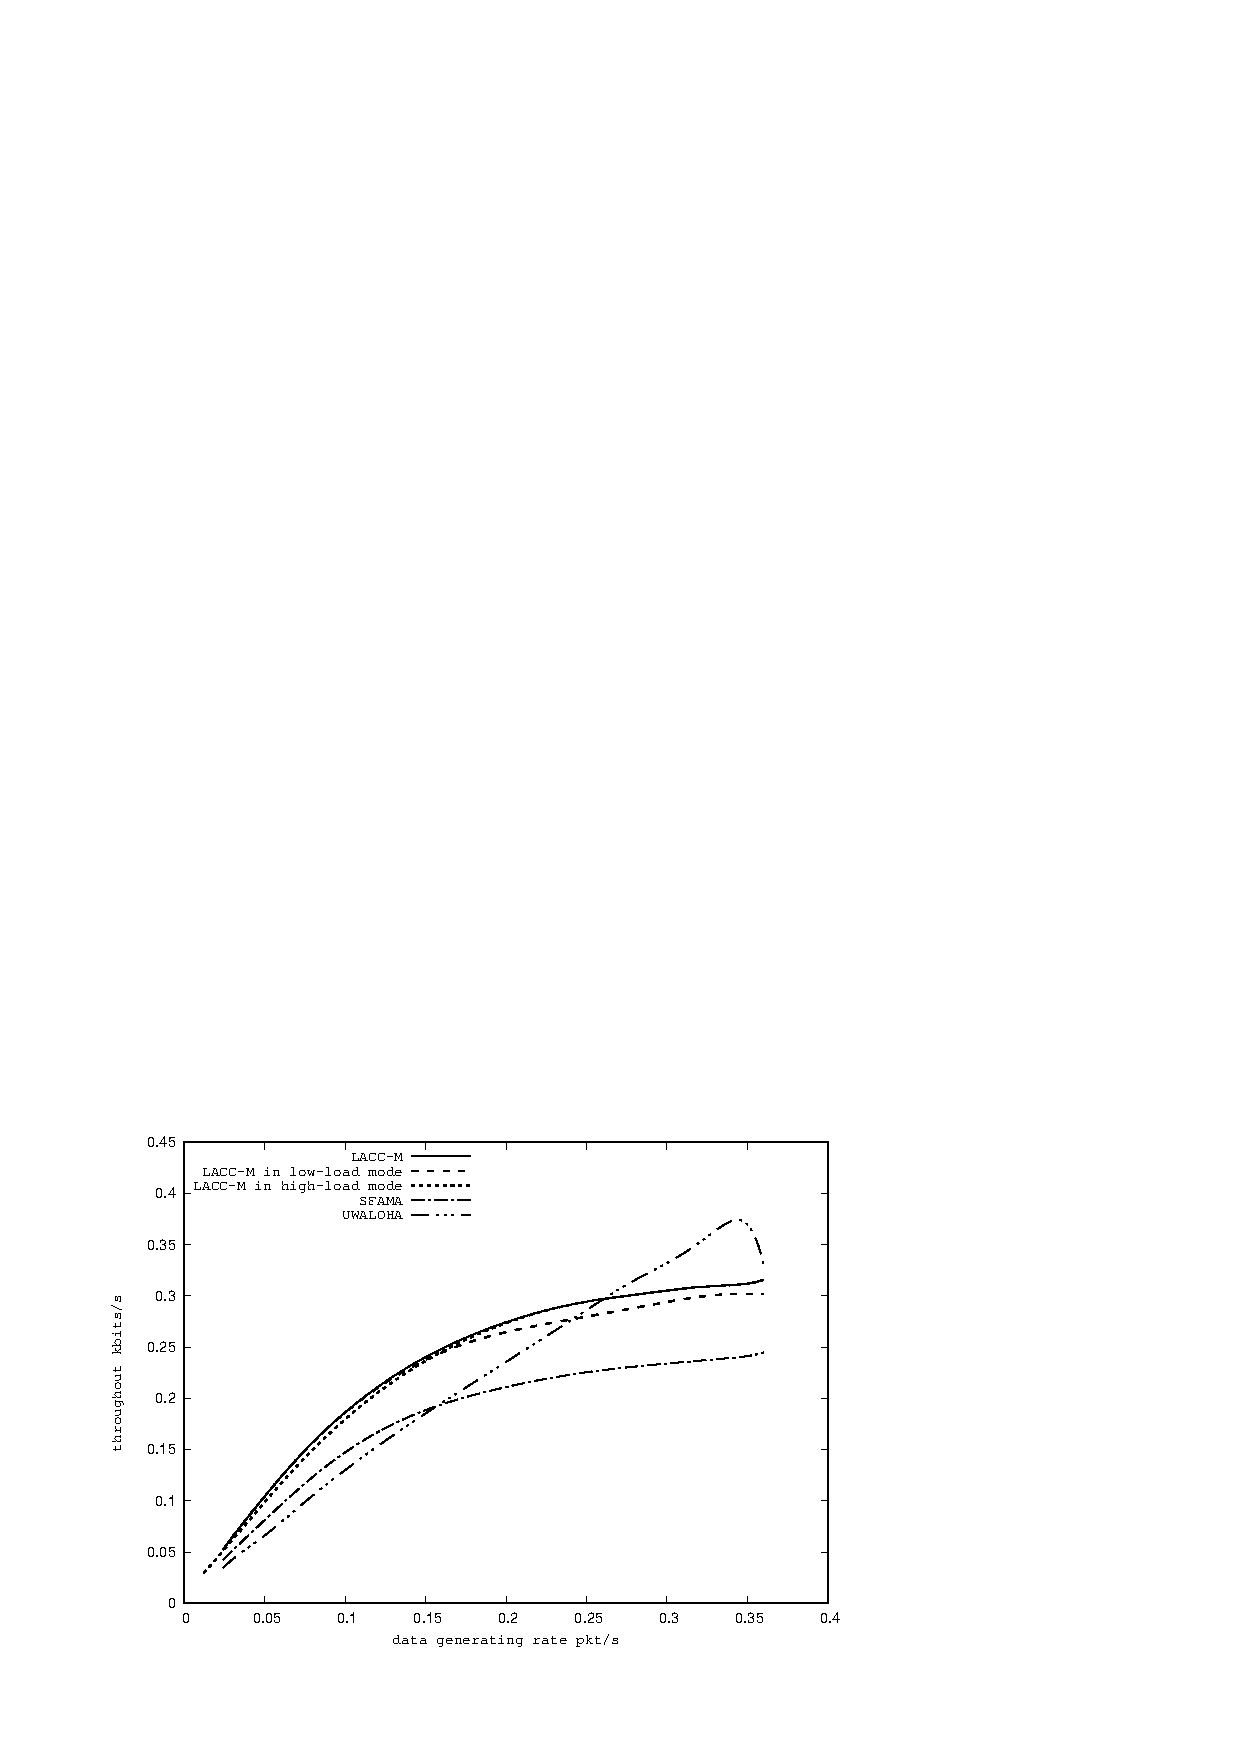
\includegraphics[scale=0.95]{figures/3nodea.pdf}
	\caption{
		吞吐量与数据产生速率关系图
	}
	\label{fig:example}
\end{figure}

和二节点移动网络相比,三节点移动网络中,单个移动节点承受的负载减少,所以高负载数据传输模式和低负载模式相比端到端时延优势减小,但仍然有所优化。
\begin{figure}[!ht]
	\centering
	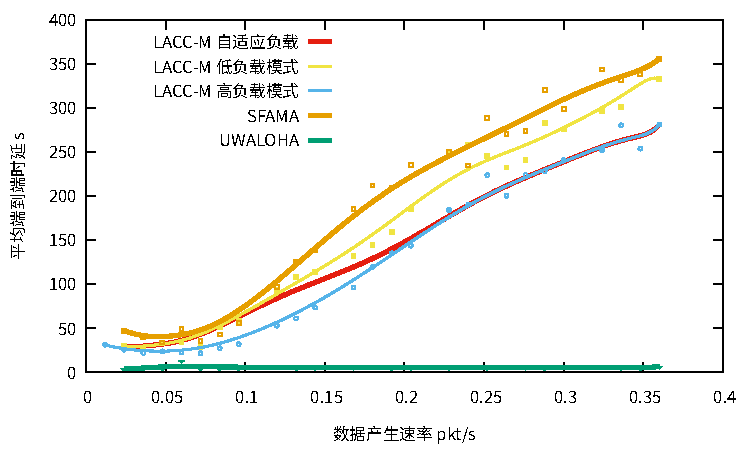
\includegraphics[scale=0.95]{figures/3nodeb.pdf}
	\caption{
		平均端到端时延与数据产生速率关系图
	}
	\label{fig:example}
\end{figure}

多加入了移动节点后,信道的利用率有所提高,所以低网络负载时的发送成功率比二移动节点模式有所提高。但是,高移动负载时,移动节点的数量增加反而会引起网络中的冲突明显增加,所以和二移动节点网络相比较,提出的LACC-M协议和SFAMA协议的发送成功率对网络负载的变化更敏感。

\begin{figure}[!ht]
	\centering
	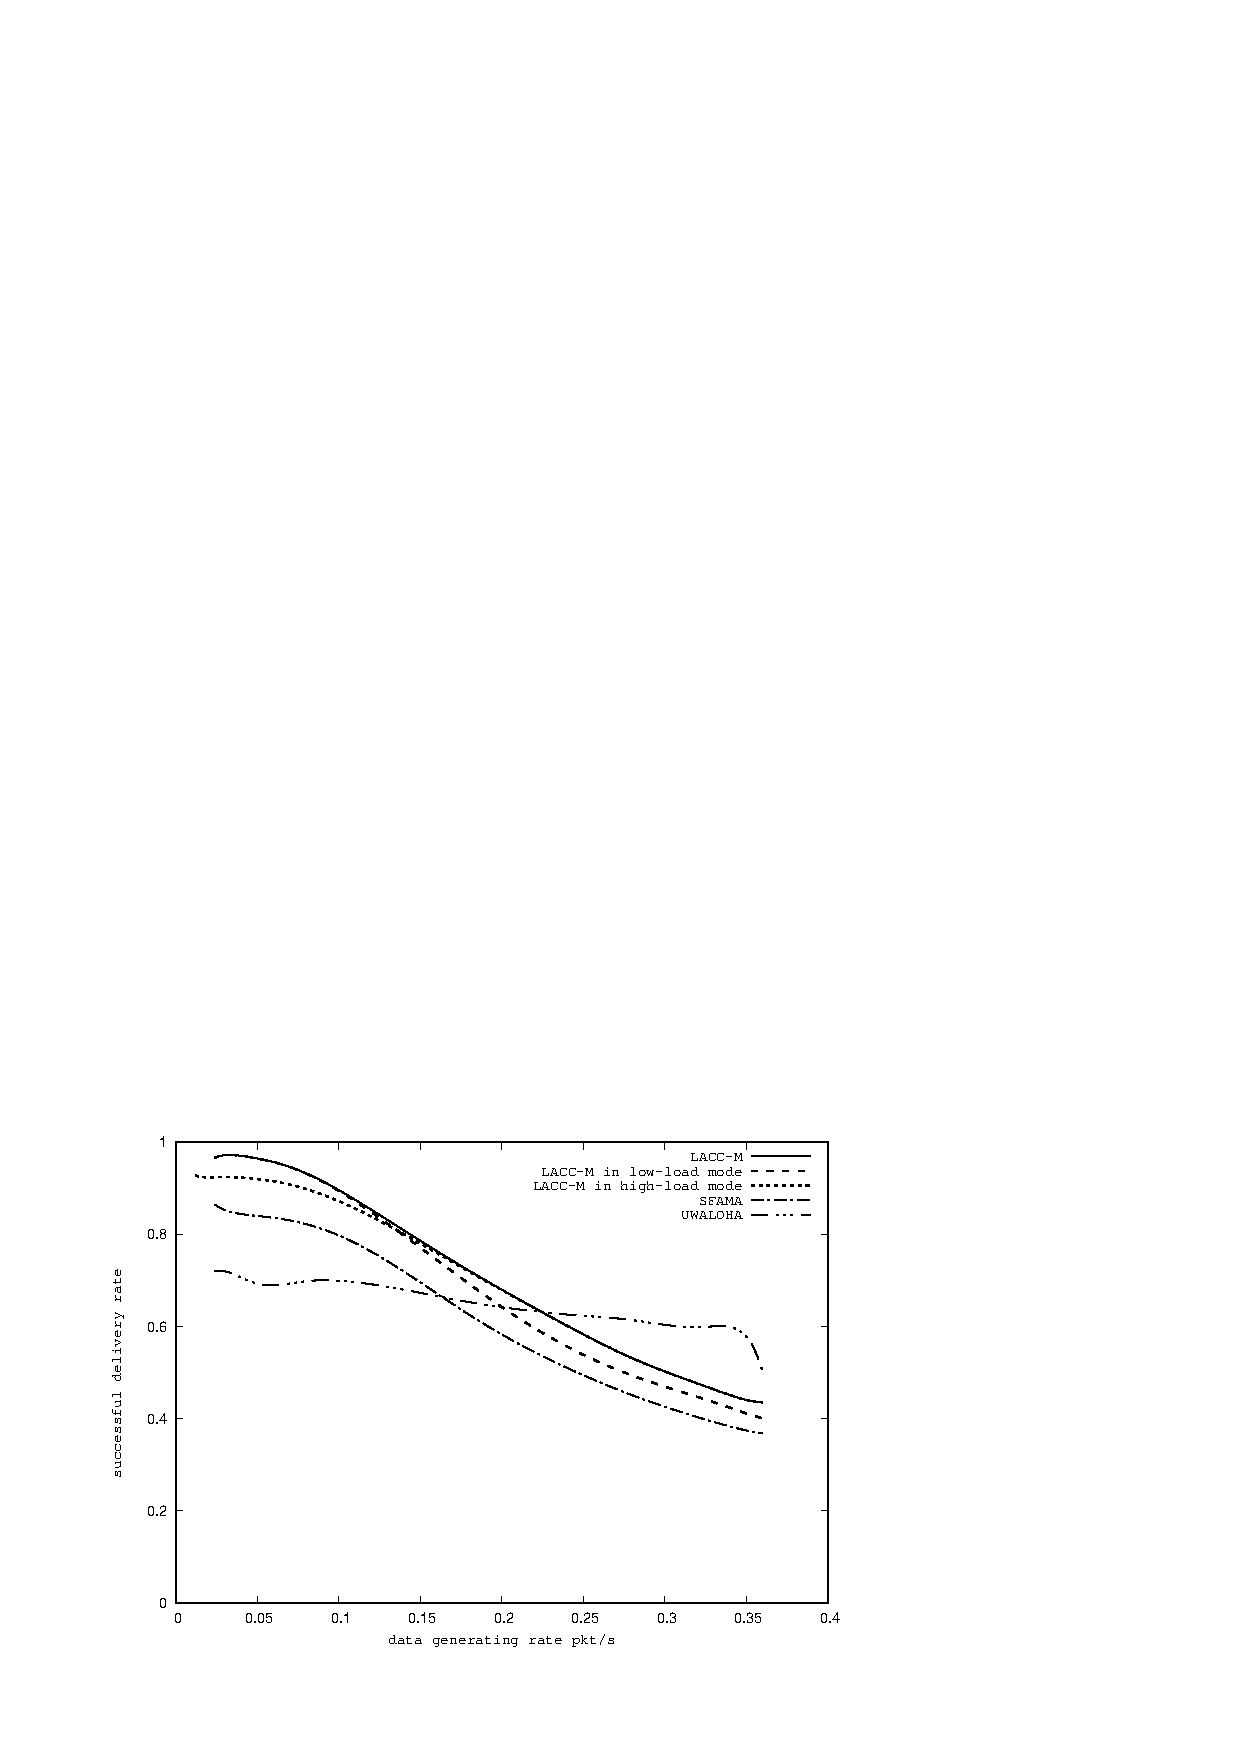
\includegraphics[scale=0.95]{figures/3nodec.pdf}
	\caption{
		发送成功率与数据产生速率关系
	}
	\label{fig:example}
\end{figure}

对于提出协议而言,多加入移动节点会带来更多的BCT帧。由于仿真时固定了SFAMA和UWALOHA的节点发送结束时间并且手动设置了目标节点,没有BCT帧的影响,所以提出协议的平均能耗偏高。

\begin{figure}[!ht]
	\centering
	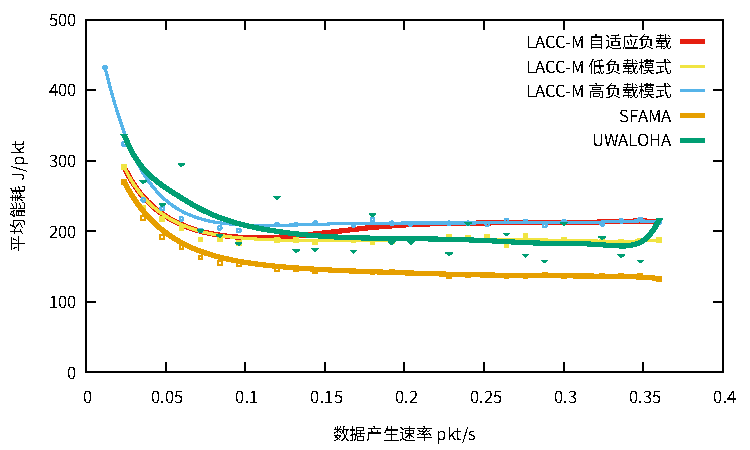
\includegraphics[scale=0.95]{figures/3noded.pdf}
	\caption{
		平均能耗与数据产生速率关系
	}
	\label{fig:example}
\end{figure}

\endinput

% 参考文献设置
\clearpage
\phantomsection
\addcontentsline{toc}{chapter}{\fHei 参考文献}
\sWuhao
% npu专用
\bibliographystyle{nputhesis}
% 参考文献位置
\bibliography{references/reference}

% 附录
\backmatter
\renewcommand{\baselinestretch}{1.5}
\fontsize{12pt}{13pt}\selectfont
\phantomsection
\chapter*{致谢}
\addcontentsline{toc}{chapter}{\fHei 致谢}
首先感谢我的导师徐文老师、陈惠芳老师和诸国磊老师。徐文老师提供了论文的研究方向和学习的平台。陈惠芳老师在论文进展过程中做了许多指点,提出了很多宝贵的意见。诸国磊老师对论文撰写过程中给拉许多指导。三位老师严谨的治学态度以及丰富的实践经验将是我以后学习和工作的动力和楷模。

同时感谢浙江大学舟山海洋研究中心的领导和同事,感谢他们提供的良好的学习和生活环境。

感谢实验室的师兄师姐,他们提供的各种资料对我帮助很大。

最后感谢我的家人和朋友一如既往的支持和关心,是他们的无私奉献和殷切希望激励着我、鞭策着我,使我能够顺利完成学业。
\clearpage
\endinput
\phantomsection
\chapter*{毕业设计小结}
\addcontentsline{toc}{chapter}{\fHei 毕业设计小结}


\clearpage
\endinput

\clearpage
\end{document}
